\documentclass[a4paper, titlepage, twoside, openright, french]{report}

\usepackage[utf8]{inputenc}
\usepackage[T1]{fontenc}
\usepackage{babel}

\usepackage{xcolor}
\usepackage{adjustbox}

\usepackage{xspace}

\usepackage{listings}
\usepackage{lstautogobble}

\usepackage{booktabs}
\usepackage{makecell}

\usepackage{fullpage}

\usepackage[hidelinks]{hyperref}

\usepackage{makeidx}
\makeindex
\usepackage[intoc]{nomencl}
\makenomenclature

\usepackage{amsmath}
\usepackage{amsthm}
\usepackage{amssymb}
\usepackage{mathtools}

\newcommand{\N}{\mathbb{N}\xspace}

\renewcommand{\epsilon}{\varepsilon}
\renewcommand{\phi}{\varphi}

\allowdisplaybreaks % Autorise les environnements à faire un page break

% J'ai suivi les recommandations de http://mirror.koddos.net/CTAN/macros/latex/required/amscls/doc/amsthdoc.pdf
\theoremstyle{plain}
\newtheorem{thm}{Théorème}[section]
\newtheorem{theorem}[thm]{Théorème} % Parce qu'à chaque fois, je me trompe
\newtheorem{lemme}{Lemme}[section]
\newtheorem{corollaire}{Corollaire}[section]

\theoremstyle{definition}
\newtheorem{definition}{Définition}[section]
\newtheorem{propriete}{Propriété}[section]
\newtheorem{exemple}{Exemple}[section]

\theoremstyle{remark}
\newtheorem{note}{Note}[section]
\newtheorem{rem}{Remarque}[section]
\newtheorem{remarque}[rem]{Remarque}
\newtheorem{illustration}{Illustration}[section]

\newenvironment{demonstration}{\begin{proof}[\textnormal{\textbf{Preuve}}]}{\end{proof}}
\newenvironment{preuve}{\begin{demonstration}}{\end{demonstration}\ignorespacesafterend}

% Traductions
\newcommand{\thmautorefname}{Théorème}
\renewcommand{\theoremautorefname}{Théorème}
\newcommand{\proprieteautorefname}{Propriété}
\newcommand{\exempleautorefname}{Exemple}
\newcommand{\lemmeautorefname}{Lemme}
\newcommand{\definitionautorefname}{Définition}
\newcommand{\algorithmautorefname}{Algorithme}
\usepackage[explicit]{titlesec}
\usepackage{chngcntr}

\counterwithin{figure}{section} % Pour que les figures soient numérotées en fonction du chapitre.section.numéro
\counterwithin{equation}{section}

% Numérotation des sous-sous-sections
\setcounter{secnumdepth}{3}
\usepackage{tikz}
\usetikzlibrary{arrows, shapes, calc, positioning, external}

\tikzexternalize
\tikzsetexternalprefix{figures/}

\tikzset {
    sum/.style = {
        draw,
        shape = circle,
        font={$\Sigma$} % Small hack to set \Sigma in every sum node
    },
    Z/.style = {
        draw,
        shape = rectangle,
        minimum width=25pt,
        minimum height=20pt,
        font = {$z^{-1}$} % To set z^{-1} in every Z node
    },
    multiply/.style args = {#1}{
        draw,
        regular polygon,
        regular polygon sides = 3,
        inner sep=0pt,
        minimum size=25pt,
        label = {[label distance=0.1cm]#1}
    },
    multiply right/.style args = {#1}{
        multiply={#1},
        shape border rotate=-90,
    },
    multiply left/.style args = {#1}{
        multiply={#1},
        shape border rotate=90,
    },
    branch/.style = {
        draw,
        shape = circle,
        fill,
        inner sep=0pt,
        minimum size=4pt
    },
    every path/.style = {
        ->,
        >=stealth',
        line width=1pt,
        draw
    }
}
\usepackage{fancyhdr}
\pagestyle{fancy}
\usepackage{emptypage}

\setlength{\headheight}{15pt}
\setlength{\headsep}{0.2cm}

\renewcommand{\chaptermark}[1]{\markboth{\thechapter. #1}{}}
\renewcommand{\sectionmark}[1]{\markright{\thesection. #1}{}}

\fancyhf{} % supprime les en-têtes et pieds prédéfinis
\fancyhead[R]{\thepage} % Met le numéro de la page à droite sur toutes les pages
\fancyhead[LE]{\textsl{\leftmark}} % Met le nom du chapitre à gauche sur les pages paires
\fancyhead[LO]{\textsl{\rightmark}} % Met le nom de la section à gauche sur les pages impaires
\renewcommand{\headrulewidth}{0.4pt}% filet en haut de page
\renewcommand{\footrulewidth}{0pt} % pas de filet en bas

\fancypagestyle{plain}{ % pages de tetes de chapitre
    \fancyhead{} % supprime l'entete
    \fancyhead[R]{\thepage}
    \renewcommand{\headrulewidth}{0pt} % et le filet
}

\linespread{1.1}

\newcommand{\transfoZ}{\xLeftrightarrow{Z}}
\newcommand{\fourier}{\xLeftrightarrow{F}}
\newcommand{\TFTD}{\xLeftrightarrow{TFTD}}

\newcommand{\NTFD}{N_{TFD}}

\newcommand{\sumInfty}[1]{\sum\limits_{#1=-\infty}^{+\infty}}
\newcommand{\intInfty}{\int_{-\infty}^{+\infty}}

\title{Formulaire et résumé de Traitement du Signal}
\date{Année académique 2018-2019}
\author{Gaëtan Staquet}

\begin{document}
    \maketitle
    \pagenumbering{roman}

    \begin{abstract}
        Ce document est un formulaire/résumé du cours de Traitement du Signal donné par Thierry Dutoit en l'année académique 2018-2019. Il est distribué sous licence MIT. Il ne vise pas à expliquer le cours mais tente de rendre le cours plus compact (en ignorant les parties purement théoriques).

        Le premier chapitre est un formulaire brut, c'est-à-dire que les formules et résultats sont donnés tels quels. Les chapitres suivants résument chacun un chapitre du cours.

        Pour rappel, le chapitre 5 du cours ne concerne pas les étudiants de la Faculté des Sciences.
    \end{abstract}

    \newpage
    \thispagestyle{fancy}
    \tableofcontents

    \newpage
    \pagenumbering{arabic}
    \documentclass[usenames,dvipsnames]{article}

\usepackage{polyglossia}
\setdefaultlanguage{french}

\usepackage{amsmath}
\usepackage{amsthm}
\usepackage{amssymb}
\usepackage{mathtools}

\newcommand{\N}{\mathbb{N}\xspace}

\renewcommand{\epsilon}{\varepsilon}
\renewcommand{\phi}{\varphi}

\allowdisplaybreaks % Autorise les environnements à faire un page break

% J'ai suivi les recommandations de http://mirror.koddos.net/CTAN/macros/latex/required/amscls/doc/amsthdoc.pdf
\theoremstyle{plain}
\newtheorem{thm}{Théorème}[section]
\newtheorem{theorem}[thm]{Théorème} % Parce qu'à chaque fois, je me trompe
\newtheorem{lemme}{Lemme}[section]
\newtheorem{corollaire}{Corollaire}[section]

\theoremstyle{definition}
\newtheorem{definition}{Définition}[section]
\newtheorem{propriete}{Propriété}[section]
\newtheorem{exemple}{Exemple}[section]

\theoremstyle{remark}
\newtheorem{note}{Note}[section]
\newtheorem{rem}{Remarque}[section]
\newtheorem{remarque}[rem]{Remarque}
\newtheorem{illustration}{Illustration}[section]

\newenvironment{demonstration}{\begin{proof}[\textnormal{\textbf{Preuve}}]}{\end{proof}}
\newenvironment{preuve}{\begin{demonstration}}{\end{demonstration}\ignorespacesafterend}

% Traductions
\newcommand{\thmautorefname}{Théorème}
\renewcommand{\theoremautorefname}{Théorème}
\newcommand{\proprieteautorefname}{Propriété}
\newcommand{\exempleautorefname}{Exemple}
\newcommand{\lemmeautorefname}{Lemme}
\newcommand{\definitionautorefname}{Définition}
\newcommand{\algorithmautorefname}{Algorithme}
\usepackage{algorithm}
\usepackage{algpseudocode}

\algblockdefx[doWhile]{DoWhile}{EndDoWhile}{\algorithmicdo}[1]{\algorithmicwhile~#1}
\algblockdefx[doUntil]{DoUntil}{EndDoUntil}{\algorithmicdo}[1]{\algorithmicuntil~#1}

\addto\captionsfrench{
    \floatname{algorithm}{Algorithme}
    \algrenewcommand\algorithmicrequire{\textbf{Entrée(s)} :}
    \algrenewcommand\algorithmicensure{\textbf{Sortie(s)} :}
    \algrenewcommand\algorithmicdo{\textbf{faire}}
    \algrenewcommand\algorithmicwhile{\textbf{tant que}}
    \algrenewcommand\algorithmicuntil{\textbf{jusqu'à ce que}}
    \algrenewcommand\algorithmicforall{\textbf{pour chaque}}
    \algrenewcommand\algorithmicfor{\textbf{pour}}
    \algrenewcommand\algorithmicend{\textbf{fin}}
    \algrenewcommand\algorithmicreturn{\textbf{retourner}}
}

\usepackage[backend = biber, style = alphabetic]{biblatex}

\addbibresource{preambule/biblio/Numerical_Analysis.bibtex}

% Pour l'index
\usepackage{makeidx}
\makeindex{}
% Pour la liste des abbréviations
\usepackage[intoc]{nomencl}
\makenomenclature
\addto\captionsfrench{
    \renewcommand{\nomname}{Liste des abbréviations}
}

\usepackage{xspace}
\usepackage{fullpage}

\usepackage{xcolor}
\usepackage{listings}
\usepackage{lstautogobble}
\lstset {
    language=R,
    commentstyle=\color{Green},
    stringstyle=\color{Orange},
    autogobble = true
}

\usepackage[hidelinks]{hyperref}
\usepackage[nameinlink]{cleveref}

\newcommand{\transfoZ}{\xLeftrightarrow{Z}}
\newcommand{\fourier}{\xLeftrightarrow{F}}
\newcommand{\TFTD}{\xLeftrightarrow{TFTD}}

\newcommand{\NTFD}{N_{TFD}}

\newcommand{\sumInfty}[1]{\sum\limits_{#1=-\infty}^{+\infty}}
\newcommand{\intInfty}{\int_{-\infty}^{+\infty}}

\title{Formulaire/Synthèse de \textit{Big Data Analytics I}}
\author{Gaëtan Staquet}
\date{Année académique 2018--2019}

\begin{document}
    \maketitle

    \begin{abstract}
        Sauf mentions contraires, toutes les informations données dans ce document proviennent des slides du cours de \textit{Big Data Analytics I} donné par M. Souhaib Ben Taieb en l'année académique 2018-2019.
    \end{abstract}

    \tableofcontents

    \clearpage
    \section{Algèbre linéaire}
    Nous donnons ici quelques formules qui pourraient être utiles. Des définitions complémentaires peuvent être trouvées dans le reste du document (comme la définition des valeurs propres). Les définitions et formules proviennent principalement de Wikipédia.

    \subsection{Signe de la dérivée seconde et maximum/minimum}
        Un point \(x\) d'une fonction \(f\) est un \textit{minimum} si \(f'(x) = 0\) et \(f''(x) > 0\).

        Un point \(x\) d'une fonction \(f\) est un \textit{maximum} si \(f'(x) = 0\) et \(f''(x) < 0\).

    \subsection{Vecteurs}
        \begin{definition}
            Soit \(q \geq 1\). La \textit{q-norme}\index{Norme} d'un vecteur \(x = (x_1, \dots, x_p)\) est
            \[
                \norm{x}_q = \left(\sum_{j=1}^p |x_j|^q\right)^{\frac{1}{q}}
            \]

            Quelques normes particulières :
            \begin{itemize}
                \item \(q = 1\): norme \(L_1\) (terme pénalisant de la régression Lasso)
                \item \(q = 2\): norme \(L_2\), norme euclidienne (terme pénalisant de la régression Ridge)
                \item \(q = \infty\): norme \(L_\infty\), norme uniforme :
                \[
                    \norm{x}_\infty = \max\{|x_1|, \dots, |x_p|\}
                \]
            \end{itemize}
        \end{definition}

        \begin{definition}
            Le \textit{produit scalaire} de deux vecteurs \(x, y \in \R^n\) est :
            \begin{align*}
                xy &= \norm{x}_2 \norm{y}_2 \cos(\theta) & \theta \text{ est l'angle entre \(x\) et \(y\)} \\
                &= \sum_{i=1}^n x_i y_i
            \end{align*}

            On peut aussi voir le produit scalaire comme un produit de deux matrices. Si on considère les deux vecteurs comme étant des vecteurs colonnes, le produit scalaire est donné par \(xy^T\).

            Le produit scalaire est commutatif et distributif.
        \end{definition}

        \begin{definition}
            Un vecteur est dit \textit{unitaire} si sa 2-norme vaut 1.

            Deux vecteurs \(x\) et \(y\) sont \textit{orthogonaux} si leur produit scalaire est nul, c'est-à-dire si \(u v = 0\).

            Deux vecteurs sont \textit{orthonormaux} s'ils sont unitaires et orthogonaux.
        \end{definition}

        \begin{definition}
            Deux vecteurs \(x, y \in \R^n\) sont \textit{linéairement dépendants} si l'un peut être exprimé comme une combinaison linéaire de l'autre, c'est-à-dire s'il existe deux scalaires \(a_1, a_2\) (non tous deux nuls, c'est-à-dire \(a_1 \not= 0 \lor a_2 \not= 0\)) tels que \(a_1 x + a_2 y = 0\) (où \(0\) est le vecteur nul).

            Deux vecteurs sont \textit{linéairement indépendants} s'ils ne sont pas linéairement dépendants.
        \end{definition}

    \subsection{Matrices}
        \begin{definition}
            Le \textit{rang} d'une matrice est le nombre de colonnes linéairement indépendantes.
        \end{definition}

        \begin{definition}
            La \textit{trace} d'une matrice carrée \(A \in \R^{n\times n}\) est 
            \[
                \trace(A) = \sum_{i=1}^n a_{ii}
            \]
        \end{definition}

        \begin{propriete}
            Soient \(A \in \R^{n \times p}, B \in \R^{p\times n}\). On a:
            \[
                \trace(AB) = \trace(BA)
            \]
        \end{propriete}

        \begin{definition}
            Le \textit{produit} de deux matrices \(A \in \R^{n \times m}, B \in \R^{m \times p}\) est la matrice \(C \in \R^{n \times p}\) telle que
            \[
                \forall i \in \{1, \dots, n\}, \forall j \in \{1, \dots, p\}, c_{ij} = \sum_{k=1}^m a_{ik} b_{kj}
            \]

            Le produit matriciel n'est pas commutatif mais est distributif et associatif.

            On a :
            \[
                (AB)^T = B^T A^T
            \]
        \end{definition}
        
        \subsection{Inverse}
            \begin{definition}
                Une matrice \(A \in \R^{n \times n}\) est dite \textit{inversible} (ou \textit{non-singulière}) si et seulement si (les conditions suivantes sont équivalentes) :
                \begin{itemize}
                    \item Son déterminant est non-nul.
                    \item Il existe une unique matrice \(B \in \R^{n \times n}\) telle que \(AB = BA = \identity_n\). \(B\) est appelé l'\textit{inverse} de \(A\) et est souvent notée \(A^{-1}\)
                    \item 0 n'est pas une valeur propre de \(A\)
                    \item Le rang de la matrice est \(n\)
                \end{itemize}
            \end{definition}

            \begin{propriete}
                On a les propriétés suivantes :
                \begin{align*}
                    (A^{-1})^{-1} &= A\\
                    \forall k \in \R\setminus\{0\}, (kA)^{-1} &= k^{-1}A^{-1}\\
                    (A^T)^{-1} &= (A^{-1})^T\\
                    \det(A^{-1}) &= (\det(A))^{-1}\\
                    (AB)^{-1} &= (B^{-1} A^{-1})
                \end{align*}
            \end{propriete}

            \subsubsection{Calculs}
                Nous donnons ici quelques formules pour calculer l'inverse d'une matrice (les formules qui semblent les plus utiles vu le reste du cours).

                \paragraph{Décomposition en valeurs propres}
                    Si une matrice peut être décomposée en valeurs propres, c'est-à-dire si on peut écrire \(A = Q \Lambda Q^T\), alors \(A\) est inversible et son inverse est donnée par :
                    \[
                        A^{-1} = Q \Lambda^{-1} Q^{-1}
                    \]
                    L'inverse de \(\Lambda\) est simple à calculer car \(\Lambda\) est une matrice diagonale.

                \paragraph{Solution analytique}
                    \begin{definition}
                        Le \textit{cofacteur} d'indice \(i,j\) de \(A\in\R^{n\times n}\) est :
                        \[
                            C_{ij} = (-1)^{i+j} \det(A_{i,j})
                        \]
                        où \(A_{i,j}\) est la sous-matrice carrée de taile \(n-1\) déduite de \(A\) en supprimant la \(i\)\ieme{} ligne et la \(j\)\ieme{} colonne.
                    \end{definition}

                    Soit \(C\), la matrice des cofacteurs de \(A\). Alors,
                    \begin{align*}
                        A^{-1} &= \frac{1}{\det(A)} C^T\\
                        (A^{-1})_{ij} &= \frac{1}{\det(A)} (C_{ji})
                    \end{align*}

                \paragraph{Matrice \(2 \times 2\)}
                    En utilisant les cofacteurs, on obtient :
                    \[
                        A^{-1} = \begin{pmatrix}
                            a & b\\
                            c & d
                        \end{pmatrix}^{-1} = \frac{1}{ad - bc} \begin{bmatrix}
                            d & -b\\
                            -c & a
                        \end{bmatrix}
                    \]
    \section{Statistiques}
    \subsection{Probabilités}
    \begin{definition}[Événement]
        Le \textit{sample space} \(\Omega\) est l'ensemble des valeurs élémentaires possibles. Par exemple, pour un lancer de pièces, les valeurs possibles sont \(\{heads, tails\}\).

        Un \textit{événement} est un sous-ensemble \(A \subseteq \Omega\). On dit qu'un événement \(A\) a lieu si le résultat d'une expérience est dans \(A\).
    \end{definition}

    \begin{definition}[Distributions]
        Une \textit{distribution de probabilités} est une fonction \(\distribution : A \to \R\). Cette fonction doit satisfaire certains axiomes :
        \begin{enumerate}
            \item Non-négative : \(\forall A \subseteq \Omega, \distribution(A) \geq 0\).
            \item Unité de \(\Omega\) : \(\distribution(\Omega) = 1\).
            \item Countable additivity : Pour une suite \(A_1, A_2, \dots\) d'ensembles disjoints, on a :
            \[
                \distribution(\bigcup_{i = 1}^\infty A_i) = \sum_{i=1}^\infty \distribution(A_i)
            \]
        \end{enumerate}

        Avec ces axiomes, il est possible de montrer les propriétés suivantes :
        \begin{itemize}
            \item \(\distribution(\emptyset) = 0\)
            \item \(\forall A, B \subseteq \Omega, A \subset B \implies \distribution(A) \leq \distribution(B)\)
            \item \(\forall A \subseteq \Omega, 0 \leq \distribution(A) \leq 1\)
            \item \(\forall A \subseteq \Omega, \distribution(\complementary{A}) = 1 - \distribution(A)\)
            \item \(\forall A, B \subseteq \Omega, \distribution(A \cup B) = \distribution(A) + \distribution(B) - \distribution(A \cap B) \Leftrightarrow \distribution(A \cap B) = \distribution (A) + \distribution(B) - \distribution(A \cup B)\)
            \item \(\implies \distribution(A \cap B) \geq \distribution(A) + \distribution(B) - 1\) car \(\distribution(A \cup B) \leq 1\)
        \end{itemize}
    \end{definition}

    \subsubsection{Probabilités conditionnelles et événéments indépendants}
        \begin{definition}
            Soient \(A, B \subseteq \Omega\), si \(\distribution(B) > 0\), alors la \textit{probabilité conditionnelle} de \(A\) étant donnée \(B\) est :
            \[
                \distribution(A | B) = \frac{\distribution(A \cup B)}{\distribution(B)}
            \]
        \end{definition}

        \begin{definition}
            Soient \(A, B \subseteq \Omega\), \(A\) et \(B\) sont dits \textit{indépendants} si 
            \[
                \distribution(A \cap B) = \distribution(A)\distribution(B)
            \]
            ou si
            \[
                \distribution(A | B) = \distribution(A)   
            \]

            Un ensemble d'événéments \(A_j (j \in I)\) sont dits \textit{mutuellement indépendants} si
            \[
                \forall J \subseteq I, \distribution\left(\bigcap_{j\in J}\right) = \prod_{j\in J} \distribution(A_j)
            \]
        \end{definition}

    \subsubsection{Règle de Bayes}
        \begin{theorem}[Loi de la probabilité totale]
            Soit \(A_1, \dots, A_k\) une partition de \(\Omega\). Alors,
            \[
                \forall B \subseteq \Omega, \distribution(B) = \sum_{i=1}^k \distribution(B | A_i) \distribution(A_i)
            \]
        \end{theorem}
        \begin{proof}
            On a que \(A_i \cap B (i = 1, \dots, k)\) forme une partition de \(B\) et \(\distribution(A_i \cap B) = \distribution(B | A_i) \distribution(A_i)\).
        \end{proof}

        \begin{theorem}[Bayes]
            Soit \(A_1, \dots, A_k\) une partition de \(\Omega\). Alors,
            \[
                \distribution(A_i | B) = \frac{\distribution(B | A_i) \distribution(A_i)}{\sum_{i=1}^k \distribution(B | A_i)\distribution(A_i)}
            \]
        \end{theorem}
    \subsection{Variables aléatoires et distributions}
    \begin{definition}
        Une \textit{variable aléatoire} est une fonction \(\Omega \to \R\). 
        
        Une façon de voir une variable aléatoire est de penser à un mapping entre une distribution sur \(\Omega\) et une distribution sur les réels (c'est-à-dire l'ensemble des valeurs de la variable aléatoire).
        Formellement, pour une variable \(X\) et un sous-ensemble \(A \in \R\) :
        \[
            \distribution_X (X \in A) = \distribution(\{\omega \in \Omega : X(\omega) \in A\})
        \]
    \end{definition}

    \begin{definition}
        Chaque variable aléatoire est associée à une \textit{fonction de distribution cumulative} (notée CDF) :
        \[
            \forall x, F_X(x) = \distribution_X(X \leq x)
        \]

        Une fonction \(F\) est une CDF si et seulement si :
        \begin{enumerate}
            \item \(\lim_{x \to -\infty} F(x) = 0\) et \(\lim_{x \to +\infty} F(x) = 1\)
            \item La fonction n'est pas décroissante en \(x\)
            \item La CDF est continue à droite, c'est-à-dire, \(\forall x_0 \in \R, \lim_{x \to x_0^+} F(x) = F(x_0)\)
        \end{enumerate}

        \(X\) est une variable continue si sa CDF est une fonction continue et est une variables discrète si sa CDF est une fonction discrète.

        Deux variables aléatoires \(X\) et \(Y\) sont identiquement distribués si \(\forall A, \distribution_X(X \in A) = \distribution_Y(Y \in A)\) (ne veut pas dire que \(X\) et \(Y\) sont égaux).

        Deux variables \(X\) et \(Y\) sont identiquement distribués si et seulement si leur CDF sont égaux, c'est-à-dire, \(\forall x, F_x(x) = F_y(x)\)
    \end{definition}

    \begin{remarque}[Notations]
        \(F_x(x)\) indique une CDF tandis que \(f_X(x)\) indique une pdf/pmf.
    \end{remarque}

    \begin{definition}
        Pour une variable discrète, sa \textit{fonction de masse} (notée \textit{PMF}) :
        \[
            f_X(x) = P_X(X = x)
        \]

        Pour une variable continue, sa \textit{densité de probabilité} (notée \textit{PDF}) \(f_X\) est la fonction qui satisfait :
        \[
            \forall x, F_X(x) = \int_{-\infty}^{x} f_X(t)\,dt
        \]

        Une fonction \(f_X(x)\) est une pdf/pmf si et seulement si :
        \begin{enumerate}
            \item \(\forall x, f_X(x) \geq 0\)
            \item \(\sum_x f_X(x) = 1\) (pour une pmf) ou \(\int_{-\infty}^{+\infty} f_X(x)\,dx = 1\) (pour une pdf)
        \end{enumerate}
    \end{definition}

    Pour trouver la probabilité qu'une variable aléatoire atterrisse dans un intervalle, il y a deux façons :
    \begin{itemize}
        \item Via les fonctions de distribution : \(\distribution(a < X \leq b) = F_X(b) - F_X(a)\)
        \item Via les fonctions de densité/de masse :
        \begin{itemize}
            \item Pour des variables continues : \(\distribution(a < X \leq b) = \int_{a}^b f_X(x)\,dx\)
            \item Pour des variables discrètes : \(\distribution(a < X \leq b) = \sum_{x > a}^{x = b} \distribution(X = x)\)
        \end{itemize}
    \end{itemize}
    \subsection{Quelques distributions}
    \subsubsection{Distributions discrètes}
        \paragraph{Distribution uniforme (discrète)}
            Sur \(k\) catégories \(\{x_1, x_2, \dots, x_k\}\), la distribution uniforme discrète est :
            \[
                \forall x \in \{x_1, x_2, \dots, x_k\}, p_X(x) = \frac{1}{k}
            \]

        \paragraph{Distribution de Bernoulli}
            Typiquement, la distribution d'un lancer de pièces, c'est-à-dire que \(x \in \{0, 1\}\). On a \(p\) qui donne la probabilité d'avoir \(1\). La pmf de Bernoulli est :
            \[
                \forall x \in \{0, 1\}, p_X(x) = p^x (1-p)^{1-x}
            \]

            Cette distribution est notée \(\bernoulli(p)\).

            Pour \(X \sim \bernoulli(p), \expectation[X] = p * 1 + (1 - p) * 0 = p\) et \(\variance[X] = p (1 - p)\).

        \paragraph{Distribution binomiale}
            Typiquement, la distribution du nombre de heads dans \(n\) lancers de pièces :
            \[
                \forall x, p_X(x) = \begin{cases}
                    \binom{n}{x} p^x (1 - p)^{n-x} & \text{si } x \in \{0, 1, \dots, n\}\\
                    0 & \text{sinon}
                \end{cases}
            \]

            Cette distribution est notée \(\binomial(n, p)\).

        \paragraph{Distribution géométrique}
            Typiquement, la distribution du nombre de lancers pour voir une face. Sa pmf :
            \[
                \forall x \in \{1, 2, \dots\}, p_X(x) = p(1-p)^{x_1}
            \]

            Cette distribution est notée \(\geometric(p)\).

        \paragraph{Distribution de Poisson}
            Une distribution de Poisson de moyenne \(\lambda\) a comme pmf :
            \[
                \forall x \in \{0, 1, \dots\}, p_X(x) = \frac{\lambda^x e^{-\lambda}}{x!}
            \]

            Cette distribution est notée \(\poisson(\lambda)\).

    \subsubsection{Distributions continues}
        \paragraph{Distribution uniforme (continue)}
            Sur \([a, b]\), sa pdf est :
            \[
                \forall x, p_X(x) = \begin{cases}
                    \frac{1}{b - a} & \text{si } x \in [a, b]\\
                    0 & \text{sinon}
                \end{cases}
            \]

            Cette distribution est notée \(\uniform[a, b]\).

        \paragraph{Distribution gaussienne}
            Cette distribution a une moyenne \(\mu\) et une variance \(\sigma^2\). Sa pdf est :
            \[
                \forall x, p_X(x) = \frac{1}{\sqrt{2\pi}\sigma} e^{-\frac{1}{2\sigma^2}(x - \mu)^2}
            \]

            Cette distribution est notée \(\gaussian(\mu, \sigma^2)\).
    \subsection{Moments, Espérance, Variance et Covariance}
    \begin{definition}
        L'\textit{espérance} ou \textit{moyenne} ou \textit{premier moment} d'une variable aléatoire \(X\) est définie par :
        \[
            \expectation[X] = \int x\,dF_X(x) = \int xf_X(x)\,dx \text{\hspace{1em}ou\hspace{1em}}  \sum_x xf_X(x)
        \]

        Si \(\expectation[X] = \infty\), on dit que l'espérance n'existe pas. % il n'y a pas d'espoir dans ce monde

        Quand le nombre d'expériences \(n\) est très grand, \(\expectation[n] \approx \frac{1}{n} \sum_{i=1}^n X_i\).
    \end{definition}

    Pour une variable aléatoire \(Y = r(X)\) (donc une transformation de \(X\)), l'espérance est donnée par la \textit{règle du statisticien fainéant} :
    \[
        \expectation[Y] = \expectation[r(X)] = \int_x r(x)\,dF_X(x)
    \]

    \begin{theorem}
        L'espérance est linéaire. En d'autres termes, pour une collection de variables aléatoires \(X_1, \dots, X_n\) et des constantes \(a_1, \dots, a_N\) :
        \[
            \expectation\left[\sum_i a_iX_i\right] = \sum_i a_i \expectation[X_i]
        \]
    \end{theorem}

    \begin{definition}
        Pour une variable aléatoire \(X\), son \textit{\(k\ieme{}\) moment} est :
        \[
            \mu_k = \expectation[X^k]
        \]

        On note généralement la moyenne par \(\mu\) au lieu de \(\mu_1\).

        Les \textit{moments centrés} sont définis par :
        \[
            \alpha_k = \expectation\left[(X - \mu)^k\right]    
        \]
    \end{definition}

    \begin{definition}
        Le second moment centré d'une variable aléatoire \(X\) est appelée sa \textit{variance}. On la note \(\sigma_X^2\). Sa racine carrée est l'\textit{écart-type}.

        On a que :
        \[
            \sigma^2_X = \expectation\left[(X - \mu)^2\right] = \expectation[X^2 + \mu^2 - 2\mu X] = \expectation[X^2] - \mu^2 \text{\hspace{2em} Par déf des moments et linéarité de \(\expectation\)}
        \]

        Pour des constantes \(a, b\), on a que :
        \[
            \sigma_{aX+b}^2 = a^2\sigma_X^2
        \]
    \end{definition}

    \begin{definition}
        La \textit{covariance} entre deux variables aléatoires \(X\) et \(Y\) est définie par :
        \[
            \covariance[X, Y] = \expectation[(X - \mu_X)(Y - \mu_Y)] = \expectation[XY] - \expectation[X]\expectation[Y]
        \]

        La covariance de deux variables aléatoires indépendantes est nulle.

        La \textit{corrélation} entre deux variables aléatoires \(X\) et \(Y\) est la forme standardisée de la covariance :
        \[
            \correlation[X, Y] = \frac{\covariance[X, Y]}{\sigma_X \sigma_Y}
        \]

        On a que \(-1 \leq \correlation[X, Y] \leq 1\).
    \end{definition}

    \begin{theorem}
        Pour des variables aléatoires \(X_1, \dots, X_n\) et des constantes \(a_1, \dots, a_n\), on a :
        \[
            \variance\left[\sum_{i=1}^n a_i X_i\right] = \sum_{i=1}^n \sum_{j=1}^n a_i a_j \covariance[X_i, X_j]
        \]
    \end{theorem}
    \begin{proof}
        On peut utiliser le résultat suivant :
        \[
            \left(\sum_{i=1}^n x_i\right)^2 = \sum_{i=1}^n \sum_{j=1}^n x_i x_j
        \]

        On a :
        \begin{align*}
            \variance\left[\sum_{i=1}^n a_i X_i\right] &= \expectation\left[\left(\sum_{i=1}^n a_i X_i - \expectation\left[\sum_{i=1}^n a_i X_i\right]\right)^2\right] & \text{Par définition de \(\variance\)}\\
            &= \expectation\left[\left(\sum_{i=1}^n a_i X_i - \sum_{i=1}^n a_i \expectation[X_i]\right)^2\right] & \text{Par linéarité de \(\expectation\)}\\
            &= \expectation\left[\left(\sum_{i=1}^n \left(a_i (X_i - \expectation[X_i])\right)\right)^2\right]\\
            &= \expectation\left[\sum_{i=1}^n \sum_{j=1}^n \left(a_i (X_i - \expectation[X_i])\right)\left(a_j \left(X_j - \expectation[X_j]\right)\right)\right] & \text{Par le résultat donné}\\
            &= \expectation\left[\sum_{i=1}^n \sum_{j=1}^n a_ia_j (X_i - \expectation[X_i])(X_j - \expectation[X_j])\right]\\
            &= \sum_{i=1}^n \sum_{j=1}^n a_i a_j \expectation\left[(X_i - \expectation[X_i])(X_j - \expectation[X_j])\right] & \text{Par linéarité de \(\expectation\)}\\
            &= \sum_{i=1}^n \sum_{j=1}^n a_i a_j \covariance[X_i, X_j] & \text{Par définition de \(\covariance\)}
        \end{align*}
    \end{proof}

    \begin{remarque}
        On peut encore simplifier cette expression. En effet, par le fait que \(\covariance[X_i, X_j] = \covariance[X_j, X_i]\) et que \(\covariance[X_i, X_i] = \variance[X_i]\), on obtient :
        \[
            \variance\left[\sum_{i=1}^n X_i\right] = \sum_{i=1}^n \variance[X_i] + 2\sum_{i=1}^n \sum_{j=i+1}^n \covariance[X_i, X_j]
        \]
    \end{remarque}

    \begin{theorem}
        Pour \(n\) variables aléatoires iid \(X_1, \dots, X_n\) :
        \[
            \variance\left[\frac{1}{n} \sum_{i=1}^n X_i\right] = \frac{1}{n^2} \sum_{i=1}^n \variance[X_i] = \frac{\sigma_X^2}{n}
        \]
    \end{theorem}
    \begin{proof}
        \begin{align*}
            \variance\left[\frac{1}{n} \sum_{i=1}^n X_i\right] &= \sum_{i=1}^n \sum_{j=1}^n \frac{1}{n^2} \covariance[X_i, X_j] & \text{Théorème précédent}\\
            &= \frac{1}{n^2} \sum_{i=1}^n \sum_{j=1}^n \covariance[X_i, X_j]\\
            &= \frac{1}{n^2} \left(\sum_{i=1}^n \variance[X_i] + 2\sum_{i=i+1}^n\sum_{j=1}^n \covariance[X_i, X_j]\right) & \text{Par la remarque précédente}\\
            &= \frac{1}{n^2} \sum_{i=1}^n \variance[X_i] & \text{Car \(X_i\) et \(X_j\) sont indépendants}
        \end{align*}
    \end{proof}

    \subsubsection{Espérance conditionnelle}
        \begin{definition}
            Soient deux variables aléatoires \(X\) et \(Y\). On veut calculer la valeur moyenne de \(Y\) quand \(X = x\). L'\textit{espérance conditionnelle} est :
            \[
                \expectation[Y | X = x] = \sum_y y f_{Y|X}(y | x) \text{\hspace{2em}ou\hspace{2em}} \expectation[Y | X = x] = \int_y y f_{Y|X}(y|x)\,dy
            \]

            L'espérance conditionnelle est une fonction en \(X\) (contrairement à l'espérance d'une variable aléatoire).
        \end{definition}

        \begin{theorem}[Indépendance]
            Si deux variables aléatoires \(X\) et \(Y\) sont indépendantes alors
            \[
                \expectation[Y | X = x] = \expectation[Y]
            \]

            En général, l'implication dans l'autre sens est fausse (des variables aléatoires dépendantes peuvent satisfaire l'expression).
        \end{theorem}

        \begin{definition}[Loi de l'espérance totale]
            Aussi appelée la \textit{tower property}, la \textit{loi de l'espérance totale} :
            \[
                \expectation_X[\expectation_{Y|X}[Y|X]] = \expectation_Y[Y]
            \]
        \end{definition}

    \subsubsection{Variance conditionnelle}
        \begin{definition}
            La \textit{variance conditionnelle} est :
            \[
                \variance[Y | X = x] = \expectation[(Y - \expectation[Y | X = x])^2 | X = x]
            \]
        \end{definition}

        \begin{definition}[Loi de la variance totale]
            La \textit{loi de la variance totale} est :
            \[
                \variance[Y] = \expectation[\variance[Y | X]] + \variance[\expectation[Y | X]]
            \]
        \end{definition}
    \subsection{Inférence statistique}
    Le but de l'inférence statistique est d'inférer des choses sur \(F\) dans \(X_1, \dots, X_n \sim F\). Il existe deux catégories de modèles statistiques :
    \begin{itemize}
        \item Modèle paramétrique : l'ensemble des distributions \(\mathcal{F}\) peut être décrit par un nombre fini de paramètres. Par exemple, un modèle gaussien peut être décrit par sa moyenne et sa variance et un modèle Bernoulli peut être décrit par son paramètre \(p\).
        \item Modèle non-paramétrique : l'ensemble des distributions \(\mathcal{F}\) ne peut pas être décrit par un nombre fini de paramètres. Par exemple, estimer directement la CDF ou la densité.
    \end{itemize}

    Pour le reste de cette section, on suppose que l'échantillon a été généré par un modèle paramétrique. On veut donc estimer les paramètres.

    \subsubsection{Méthode des moments}
        Supposons qu'il y a \(k\) paramètres à estimer \(\theta = (\theta_1, \dots, \theta_K)\). On peut estimer \(\theta\) en trouvant \(k\) moments. Soient
        \[
            m_1 = \frac{1}{n} \sum_{i=1}^n X_i, m_2 = \frac{1}{n} \sum_{i=1}^n X_i^2, \dots, m_k = \frac{1}{n} \sum_{i=1}^n X_i^k
        \]

        Soit \(\mu_i(\theta) = \int x^i p_\theta(x)\,dx\) le moment du \(i\ieme{}\) individu. La \textit{méthode des moments} consiste à résoudre le système suivant :
        \[
            \begin{cases}
                m_1 &= \mu_1(\theta_1, \dots, \theta_k)\\
                &\vdots\\
                m_k &= \mu_k(\theta_1, \dots, \theta_k)
            \end{cases}
        \]

    \subsubsection{Maximum Likelihood Estimation}
        Supposons que \(X_1, \dots, X_n \sim p_\theta\) avec \(p_\theta\) la pmf ou la pdf.

        \begin{definition}
            La fonction \textit{likelihood}\index{Likelihood} est définie par :
            \[
                L(\theta) \equiv L(\theta, X_1, \dots, X_n) = \prod_{i=1}^n p_\theta(X_i)
            \]

            La fonction \textit{log-likelihood} est définie par :
            \[
                l(\theta) \equiv l(\theta, X_1, \dots, X_n) = \log(L(\theta))
            \]

            Le \textit{Maximum Likelihood Estimator} (noté \textit{MLE}\index{MLE})\nomenclature{MLE}{Maximum Likelihood Estimator (ou Estimation)} est la valeur de \(\theta\) qui maximise \(L(\theta)\) (et \(l(\theta)\) car le \(\log\) est une fonction croissante). Cette valeur est notée \(\estimation{\theta}\) :
            \[
                \estimation{\theta} = \argmax_\theta L(\theta) = \argmax_\theta l(\theta)
            \]
        \end{definition}

        Typiquement, on calcule le MLE en dérivant partiellement \(l(\theta)\). En d'autres termes, on résoud le système d'équations :
        \[
            \forall i \in \{1, \dots, k\}, \frac{\partial}{\partial \theta_i} l(\theta) = 0
        \]
    \section{Apprentissage supervisé}
    \subsection{Éléments communs}
        \begin{definition}
            Les \textit{variables d'entrée}\index{Variable!d'entrée} (\textit{input variables}\index{Input variable|see {Variable, d'entrée}}), aussi appelées \textit{predictors}\index{Predictor|see {Variable, d'entrée}}, \textit{variables indépendantes}\index{Variable!indépendante|see {Variable, d'entrée}}, \textit{features}\index{Feature|see {Variable, d'entrée}} ou simplement \textit{variables}, sont représentées par le symbole \(X\). S'il y a \(p\) variables différentes, on écrit :
            \[X = (X_1, X_2, \dots, X_p)\]
        \end{definition}

        \begin{remarque}
            \(X\) est une variable aléatoire. Une réalisation de cette variable (comme, par exemple, une instance dans un jeu de données) est notée \(x\).
        \end{remarque}

        \begin{definition}
            La \textit{variable de sortie}\index{Variable!de sortie} (\textit{output variable}\index{Output variable|see {Variable, de sortie}}), aussi appelée \textit{réponse}\index{Réponse|see {Variable, de sortie}} ou \textit{variable dépendante}\index{Variable!dépendante|see {Variable, de sortie}} est souvent notée \(Y\).
        \end{definition}

        On suppose qu'il existe une relation aléatoire entre \(X\) et \(Y\), c'est-à-dire :
        \[\distribution(X, Y) = \distribution(X)\distribution(Y|X) \not= \distribution(X)\distribution(Y)\]

        \begin{definition}
            Les \textit{données}\index{Données} :
            \[
                \data = \{(x_1, y_1), (x_2, y_2), \dots, (x_n, y_n)\} = \{(x_i, y_i\}^n_{i=1}
            \]
            où \(x_i = (x_{i,1}, \dots, x_{i,p})\), c'est-à-dire que \(x_i\) est le tuple des variables pour la i\ieme{} instance (ligne) dans les données.

            On peut voir les données comme un échantillon i.i.d. de la véritable distribution, c'est-à-dire :
            \[(x_i, y_i) \stackrel{i.i.d.}{\sim} \distribution(X, Y)\]
            \nomenclature{i.i.d.}{Indépendant et identiquement distribué}
        \end{definition}

        On peut décrire tous les problèmes d'apprentissage supervisé avec les éléments suivants :
        \begin{itemize}
            \item Les \textit{variables d'entrée}\index{Variable!d'entrée} \(X\) et la \textit{variable de sortie}\index{Variable!de sortie} \(Y\);
            \item Les \textit{données}\index{Données} \(\data = \{(x_i, y_i)_{i=1}^n\}\);
            \item La \textit{fonction cible}\index{Fonction!cible}. Par exemple, la distribution jointe \(\distribution(X, Y)\), l'espérance conditionnelle \(\expectation[Y|X]\), la distribution conditionnelle \(\distribution(Y|X)\), etc.;
            \item L'\textit{ensemble d'hypothèses}\index{Ensembles d'hypothèses} \(\hypo\) contient toutes les hypothèses à considérer (les fonctions à tester). Souvent, cet ensemble est défini implicitement; et
            \item La \textit{fonction de perte}\index{Fonction!de perte} (ou \textit{fonction de coût}\index{Fonction!de coût|see {Fonction, de perte}}) \(L(y, \estimation{y})\) est une fonction \(\R \times \R \to \R^+\). Par exemple, \(L(y, \estimation{y}) = (y - \estimation{y})^2\).
        \end{itemize}
        L'\textit{algorithme d'apprentissage}\index{Algorithme!d'apprentissage} choisi la meilleure hypothèse de \(\hypo\) en utilisant les données \(\data\) et la fonction de perte \(L\).

        \subsubsection{Erreurs}
            \begin{definition}
                L'\textit{erreur de test}\index{Erreur!de test} (ou \textit{erreur out-of-sample}\index{Erreur!out-of-sample|see {Erreur, de test}}) de l'hypothèse \(\fEstimated\) permet de tester la performance de l'hypothèse sur de nouvelles données et est défini par :
                \[
                    \errorOut(\fEstimated) = \expectation[L(Y, \fEstimated(X))]
                \]
            \end{definition}

            On veut sélectionner la meilleure hypothèse :
            \[
                \fEstimated = \argmin_{h \in \hypo} \errorOut(\widehat{h}_\data)
            \]

            Cependant, on ne sait pas calculer \(\errorOut(\fEstimated)\) car on ne connait pas \(\distribution(Y, X)\).

        \subsubsection{Biais et variance}
            \begin{definition}
                Le \textit{biais}\index{Biais} est l'erreur introduite en modélisant un problème compliqué par un problème plus simple.

                La \textit{variance}\index{Variance} permet de mesurer à quel point le modèle construit serait différent si les données d'entraînement étaient différentes.
            \end{definition}

            En général, une méthode plus flexible implique un biais plus petit et une variance plus grande (car la méthode colle mieux aux données d'entraînement).

            \begin{remarque}
                La taille de l'ensemble d'entraînement a un impact sur la variance. Un plus grand ensemble réduit la variance !
            \end{remarque}

    \section{Régression avancée}
    Rappel : solution optimale de la régression linéaire donnée par OLS : \(\betaLS = (X^TX)^{-1} X^Ty\)

    Cette solution peut avoir des problèmes en haute dimension parce qu'il peut arriver que certaines colonnes de \(X\) ne sont pas linéairement indépendantes. Par conséquent, \(X\) n'est pas `full rank'. Dans ce cas, \(X^T X\) est singulière (non-inversible) et les coefficients OLS n'ont pas une unique valeur.

    Pour rappel, le biais de \(\betaLS\) est \(\expectation[\betaLS] - \beta^* = 0\) et la variance est \(\variance[\betaLS] = \sigma^2 (X^T X)^{-1}\). Si \(X\) a des colonnes orthonormales :
    \[
        \trace(\variance[\betaLS]) = \sigma^2 p
    \]

    On peut réduire le nombre de dimensions en appliquant PCA (dans ce cas, on fait du \textit{principal components regression} ou PCR\index{PCR}). Ceci suppose que les directions dans lesquels \(X_1, \dots, X_p\) ont la plus grande variation ont une relation avec \(Y\).

    Une autre solution est d'utiliser le \textit{best subset selection}\index{Best subset selection} :
    \begin{align*}
        &\min_{\beta} \left\{\sum_{i=1}^n \left(y_i - \beta_0 - \sum_{j=1}^p \beta_j x_{ij}\right)^2\right\}\\
        &\text{sous contrainte } \sum_{j=1}^p \identity(\beta_j \not= 0) \leq s
    \end{align*}
    avec \(s \geq 0\) un hyper-paramètre. Il faut considérer \(p \choose s\) modèles contenant \(s\) prédicteurs. Ceci est infaisable quand \(p\) et \(s\) sont grands. De plus, quand l'espace de recherche est grand, il y a de grands risques d'overfitting. On peut utiliser les stepwise procedures pour contrecarrer ça (mais ces méthodes ne garantissent pas d'obtenir l'optimal).

    \subsection{Shrinkage}
        Finalement, la dernière solution du cours est le \textit{shrinkage}\index{Shrinkage}.
        \begin{definition}
            Le \textit{shrinkage} (ou \textit{regularization}\index{Regularization|see {Shrinkage}}) consiste à fitter un modèle utilisant les \(p\) variables mais les coefficients estimés sont réduits vers zéro par rapport aux coefficients de OLS. Ceci a pour effet de réduire la variance et de faire de la sélection de variables.
        \end{definition}

        \subsubsection{Ridge regression}
            \begin{definition}
                La \textit{régression Ridge}\index{Ridge} est le problème d'optimisation suivant :
                \begin{align*}
                    &\min_{\beta} \left\{\sum_{i=1}^n \left(y_i - \beta_0 - \sum_{j=1}^p \beta_j x_{ij}\right)^2\right\}\\
                    &\text{sous contrainte } \sum_{j=1}^p \beta_j^2 \leq s
                \end{align*}
                avec \(s \leq 0\) un hyper-paramètre.

                Si \(s = 0\), \(\betaRidge = (0, \dots, 0)\). Si \(s = +\infty, \betaRidge = \betaLS\). Si \(s \in ]0, +\infty[\), on fait du tradeoff.
            \end{definition}

            Géométriquement, la contrainte de régularisation est une sphère.

            \begin{definition}
                On peut formuler la régression ridge comme :
                \[
                    \min_{\beta} \sum_{i=1}^n \left(y_i - \beta_0 - \sum_{j=1}^p \beta_j x_{ij}\right)^2 + \lambda \sum_{j=1}^p \beta_j^2
                \]
                avec \(\lambda \leq 0\) un hyper-paramètre.

                Si \(\lambda = 0\), \(\betaRidge = \betaLS\). Si \(\lambda = \infty\), \(\betaRidge = (0, \dots, 0)\). Si \(\lambda \in (0, \infty)\), on fait du tradeoff.

                On peut résoudre ce problème par augmentation des données :
                \[
                    \betaRidge = (X^T X + \lambda \identity_p)^{-1} X^T y
                \]
            \end{definition}

            \paragraph{Un cas simple}
                Supposons que \(n = p\) et que \(X = \identity_n = \identity_p\), alors :
                \begin{align*}
                    &\min_\beta \sum_{j=1}^p (y_j - \beta_j)^2 &\implies \betaLS &= y_j\\
                    &\min_\beta \sum_{j=1}^p (y_j - \beta_j)^2 + \lambda\sum_{j=1}^p \beta_j^2 &\implies \betaRidge &= \frac{y_j}{1+\lambda} = \frac{\betaLS}{1 + \lambda}
                \end{align*}

            \paragraph{Scaling}
                Les coefficients OLS sont `scale equivariant' (multiplier \(X_j\) par une constante \(c \implies\) les coefficients OLS sont divisés par \(c\); peu importe comment la \(j\)\ieme{} variable est scalée, \(X_j\betaEstimated{j}\) est toujours le même). En revanche, les coefficients Ridge peuvent changer drastiquement (à cause de la somme des coefficients au carré).

            \paragraph{Biais et variance}
                Posons \(R = X^T X\)
                \begin{align*}
                    \betaRidge &= (X^T X + \lambda \identity_p)^{-1} X^T y = (R + \lambda \identity_p)^{-1} R(R^{-1} X^T y)\\
                    &= (R + \lambda \identity_p)^{-1} R \betaLS = \left[R(\identity_p + \lambda R^{-1})\right]^1 R \betaLS\\
                    &= (\identity_p + \lambda R^{-1})^{-1} \betaLS
                \end{align*}
                
                Posons \(W_\lambda = (\identity_p + \lambda R^{-1})^{-1}\)
                \begin{align*}
                    \expectation[\betaRidge] &= \expectation[W_\lambda \betaLS] = W_\lambda B \not= \beta & \text{Si \(\lambda \not= 0\)}\\
                    \variance[\betaRidge] &= \variance[W_\lambda \betaLS] = W_\lambda \variance[\betaLS] W_\lambda^T \leq \variance[\betaLS]
                \end{align*}
                On a donc un biais mais un plus petite variance.

            \paragraph{Décomposition en valeurs singulières}
                On peut utiliser la décomposition en valeurs singulières\index{SVD}, c'est-à-dire \(X = U D V^T\). Donc,
                \begin{align*}
                    X^T X &= (UDV^T)^T UDV^T\\
                    &= VD^TU^T UDV^T\\
                    &= VD^T DV^T & \text{Car les colonnes de \(U\) sont orthonormales}\\
                    &= V D^2 V^T & \text{Car \(D\) est diagonale}\\
                    \\
                    \betaLS &= (X^T X)^{-1} X^T y & \text{Définition}\\
                    &= V D^{-1} U^T y & X = U D V^T \text{ et \(V^{-1} = V^T\) (car colonnes orthonormales)}\\
                    &= V D^{-2} D U^T y\\
                    \betaRidge &= (X^T X + \lambda \identity_p)^{-1} X^T y & \text{Définition}\\
                    &= (V D^2 V^T + \lambda VV^T)^{-1} VDU^T y & VV^T = \identity_p \text{ car colonnes orthonormales}\\
                    &= (V(D^2 + \lambda \identity_p) V^T)^{-1} V D U^T y\\
                    &= V(D^2 + \lambda \identity_p)^{-1} V^T V D U^T y\\
                    &= V(D^2 + \lambda \identity_p)^{-1} D U^T y
                \end{align*}
                Les deux expressions ont quasiment la même formulation à une différence près : \(+ \lambda\) pour Ridge. On peut aussi déterminer l'expression des \(\estimation{y}\) :

                \begin{align*}
                    \yLS &= X \betaLS\\
                    &= U D V^T V D^{-2} D U^T y\\
                    &= U D D^{-2} D U^T y\\
                    &= U U^T y\\
                    \yRidge &= X\betaRidge\\
                    &= X V (D^2 + \lambda \identity_p)^{-1} D U^T y\\
                    &= U D V^T V (D^2 + \lambda \identity_p)^{-1} D U^T y\\
                    &= U D (D^2 + \lambda \identity_p)^{-1} D U^T y\\
                    &= U \diagonal(\frac{d_j^2}{d_j^2 + \lambda}) U^T y & \text{\(D\) est diagonale}
                \end{align*}

                Comme \(\lambda \geq 0\), on a \(\frac{d_j^2}{d_j^2 + \lambda} \leq 1\). On a donc bien un effet de shrinkage. Quand \(d_j^2\) est petit, le shrinkage est plus important. La variable \(z_j = X v_j = u_j d_j\) est la \(j\)\ieme{} PC de \(X\).

        \subsubsection{Lasso}
            \begin{definition}
                La \textit{régression Lasso}\index{Lasso}\nomenclature{Lasso}{Least absolute shrinkage and selection operator} est le problème d'optimisation :
                \begin{align*}
                    &\min_\beta \left\{\sum_{i=1}^n \left(y_i - \beta_0 - \sum_{j=1}^p \beta_j x_{ij}\right)^2\right\}\\
                    &\text{sous contrainte} \sum_{j=1}^p |\beta_j| \leq s
                \end{align*}
                avec \(s \geq 0\) un hyper-paramètre.

                Notons \(\betaLasso\) l'estimation des coefficients pour la régression Lasso.

                Si \(s = 0, \betaLasso = (0, \dots, 0)\). Si \(s = \infty, \betaLasso = \betaLS\). Si \(s \in ]0, \infty[\), on fait du tradeoff.
            \end{definition}

            \begin{definition}
                De manière équivalente, on peut exprimer la régression Lasso comme :
                \[
                    \min_\beta \sum_{i=1}^n \left(y_i - \beta_0 - \sum_{j=1}^p \beta_j x_{ij}\right)^2 + \lambda \sum_{j=1}^p |\beta_j|
                \]
                où \(\lambda \geq 0\) est un hyper-paramètre.

                Si \(s = 0, \betaLasso = \betaLasso\). Si \(s = \infty, \betaLasso = (0, \dots, 0)\). Si \(s \in ]0, \infty[\), on fait du tradeoff.
            \end{definition}

            \paragraph{Un cas simple}
                Supposons que \(n = p\) et que \(X = \identity_p = \identity_n\). Dans ce cas, la régression Lasso est 
                \[
                     \min_\beta \sum_{j=1}^p (y_j - \beta_j)^2 + \lambda \sum_{j=1}^p |\beta_j|
                \]
                Alors, on a :
                \[
                    \betaLasso_j = \begin{cases}
                        y_j - \frac{\lambda}{2} & \text{si } y_j > \frac{\lambda}{2}\\
                        y_j + \frac{\lambda}{2} & \text{si } y_j < \frac{-\lambda}{2}\\
                        0                       & \text{si } |y_j| \leq \frac{\lambda}{2}
                    \end{cases}
                \]

                La régression Lasso shrink les coefficients OLS vers zéro par la même constante \(\frac{\lambda}{2}\) et entièrement vers zéro quand ces coefficients sont plus petits que \(\frac{\lambda}{2}\) en valeur absolue.
    \subsection{Classification}
    \begin{lstlisting}
        # Régression logistique
        glm(formule, data = data, family = binomial)
        # LDA
        lda(formule, data = data)
        # QDA
        qda(formule, data = data)
        # k-NN (attention, il faut avoir train.X, train.y et test.X)
        knn(train.X, test.X, train.y, k = 1)
        # Arbres
        tree(formule, data = data)
        # Forêts aléatoires en utilisant m variables et n arbres
        randomForest(formule, data = data, mtry = m, ntrees = n)
    \end{lstlisting}

    \subsubsection{Récupérer probabilités}
        \lstinline{predict} supporte le paramètre \lstinline{type = "prob"} pour récupérer les probabilités pour certains modèles. Pour d'autres (comme \lstinline{glm}), il faut \lstinline{type = "response"}.
    \section{Sélection de modèle}
    \begin{definition}
        La \textit{procédure de sélection de modèle} :
        \begin{enumerate}
            \item Génération des modèles : on génère un ensemble des modèles à essayer.
            \item Validation des modèles : on évalue la performance des modèles en calculant l'erreur de validation, c'est-à-dire une estimation de l'erreur de test.
            \item Sélection d'un modèle : on choisit un modèle. Typiquement, on prend celui qui minimise l'erreur de validation.
        \end{enumerate}
    \end{definition}

    \subsection{Erreurs de training vs de test pour la régression}
        Prenons la régression linéaire. Les paramètres sont estimés par \(\betaEstimated{} = (X^TX)^{-1}X^Ty\), c'est-à-dire la solution OLS\index{OLS}. Les réponses de la régression sont données par :
        \[\estimation{y} = X\betaEstimated{} = X(X^TX)^{-1} X^T y = Hy\]
        avec \(H = X(X^T X)^{-1} X^T\) la \textit{matrice hat}\index{Hat matrix}.

        Pour la régression, \(\betaEstimated{}\) est calculé en minimisant le training MSE\index{MSE}. Notons aussi \(\widetilde{\beta}\) l'estimation obtenue avec le test MSE.
        
        \begin{theorem}[Espérances et MSE]
            On a que :
                \[
                    \expectation\left[\frac{1}{n}\sum_{i=1}^n \left(y_i - \betaEstimated{}^T x_i\right)^2\right] \leq \expectation\left[\frac{1}{m} \sum_{i=1}^m \left(\widetilde{y_i} - \betaEstimated{}^T \widetilde{x_i}\right)^2\right]
                \]

            En d'autres termes, l'espérance du training MSE est inférieure ou égale à l'espérance du test MSE.
        \end{theorem}
        \begin{proof}
            On a que \(\expectation\left[\frac{1}{m} \sum_{i=1}^m \left(\widetilde{y_i} - \betaEstimated{}^T \widetilde{x_i}\right)^2\right] = \expectation\left[\frac{1}{n} \sum_{i=1}^n \left(\widetilde{y_i} - \betaEstimated{}^T \widetilde{x_i}\right)^2\right]\) car le nombre de points ne change pas l'espérance.

            Par facilité, notons \(A = \frac{1}{n}\sum_{i=1}^n \left(y_i - \betaEstimated{}^T\right)^2\) et \(B = \frac{1}{n} \sum_{i=1}^n \left(\widetilde{y_i} - \widetilde{\beta}^T \widetilde{x_i}\right)^2\) (attention au fait que le \(\beta\) de \(B\) a un tilde et non un chapeau !).

            \(A\) et \(B\) ont la même distribution (vu que \(\{(y_i, x_i)\}_{i=1}^n\) et \(\{(\widetilde{y_i}, \widetilde{x_i})\}_{i=1}^n\) suivent la même distribution). Donc, \(\expectation[A] = \expectation[B]\).

            \(B = \frac{1}{n}\sum_{i=1}^n \left(\widetilde{y_i} - \widetilde{\beta}^T \widetilde{x_i}\right)^2 \leq \frac{1}{n} \sum_{i=1}^n \left(\widetilde{y_i} - \betaEstimated{}^T \widetilde{x_i}\right)^2\) par optimalité de l'estimation OLS.

            Donc, \(\expectation[B] \leq \expectation\left[\frac{1}{n} \sum_{i=1}^n (\widetilde{y_i} - \betaEstimated{}^T \widetilde{x_i})^2\right]\).

            Finalement, on a \(\expectation[A] = \expectation[B]\) et \(\expectation[B] \leq \expectation\left[\frac{1}{n} \sum_{i=1}^n (\widetilde{y_i} - \betaEstimated{}^T \widetilde{x_i})^2\right]\). Donc :
            \[
                \expectation\left[\frac{1}{n} \sum_{i=1}^n (y_i - \betaEstimated{}^T x_i)^2\right] = \expectation\left[\frac{1}{m} \sum_{i=1}^m (\widetilde{y_i} - \betaEstimated{}^T \widetilde{x_i})^2\right]
            \]
        \end{proof}

        On veut avoir la plus petite erreur de test pour un nouveau point aléatoire \((x_0, y_0)\) où \(x_0\) et \(y_0\) sont aléatoires. On peut simplifier ce problème. On va garder les mêmes \(x\) mais générer de nouveaux \(y\) bruités. Donc, on fit le modèle sur \(y_i = x_i^T\beta + \varepsilon_i\) mais on prédit sur des échantillons générés comme \(y_i' = x_i^T\beta + \varepsilon_i'\) où \(\varepsilon_i\) et \(\varepsilon_i'\) sont iid. On va tester si le modèle entraîné sur \((x_i, y_i)\) donne des bonnes prédictions pour \((x_i, y_i')\).

        Soit \(\estimation{m_i} = x_i \betaEstimated{}\). On veut comparer \(\expectation\left[\frac{1}{n} \sum_{i=1}^n (y_i' - \estimation{m_i})^2\right]\) avec \(\expectation\left[\frac{1}{n} \sum_{i=1}^n (y_i - \estimation{m_i})^2\right]\). Remarquons que \(y_i\) et \(\estimation{m_i}\) sont des variables aléatoires dépendantes (pas indépendantes) puisque \(\estimation{m_i}\) dépend de \(y_i\) (à travers \(\betaEstimated{}\)). En revanche, \(y_i'\) et \(\estimation{m_i}\) sont indépendants.

        On a :
        \begin{align*}
            \expectation\left[(y_i - \estimation{m_i})^2\right] &= \variance[y_i - \estimation{m_i}] + (\expectation[y_i - \estimation{m_i}])^2 & \text{Car } \variance^2[X] = \expectation[X^2] - \expectation^2[X]\\
            &= \variance[y_i] + \variance[\estimation{m_i}] - 2\covariance[y_i, \estimation{m_i}] + (\expectation[y_i] - \expectation[\estimation{m_i}])^2 & \text{Propriétés variance et espérance}\\
            \expectation\left[(y_i' - \estimation{m_i})^2\right] &= \variance[y_i' - \estimation{m_i}] + (\expectation[y_i' - \estimation{m_i}])^2\\
            &= \variance[y_i'] + \variance[\estimation{m_i}] - 2\covariance[y_i', \estimation{m_i}] + (\expectation[y_i'] - \expectation[\estimation{m_i}])^2
        \end{align*}

        \(y_i\) et \(y_i'\) sont indépendants mais ont la même distribution. Donc, \(\expectation[y_i] = \expectation[y_i']\) et \(\variance[y_i] = \variance[y_i']\). On a aussi que \(\covariance[y_i', \estimation{m_i}] = 0\) (car variables indépendantes).

        Donc :
        \begin{align*}
            \expectation\left[(y_i' - \estimation{m_i})^2\right] &= \variance[y_i] + \variance[\estimation{m_i}] + (\expectation[y_i] - \expectation[\estimation{m_i}])^2 = \expectation\left[(y_i - \estimation{m_i})^2\right] + 2\covariance[y_i, \estimation{m_i}]\\
            \expectation\left[\frac{1}{n} \sum_{i=1}^n (y_i' - \estimation{m_i})^2\right] &= \expectation\left[\frac{1}{n} \sum_{i=1}^n (y_i - \estimation{m_i})^2\right] + \frac{2}{n} \sum_{i=1}^n \covariance[y_i, \estimation{m_i}]\\
            &\approx \frac{1}{n} \sum_{i=1}^n (y_i - \estimation{m_i})^2 + \frac{2}{n} \sum_{i=1}^n \covariance[y_i, \estimation{m_i}]
        \end{align*}

        \begin{definition}
            Le training error sous-estime systématiquement le test error. L'\textit{optimisme}\index{Optimisme} est la mesure de ce qui est sous-estimé.

            Une façon d'estimer le test error est d'estimer l'optimisme et de l'ajouter au training error (voir AIC et BIC)\index{AIC}\index{BIC}.

            Une autre façon est de directement estimer le test error via des méthodes de resampling\index{Resampling} (voir validation set, cross-validation et bootstrap).
        \end{definition}

        \begin{exemple}
            Pour la régression linéaire, supposons que \(X \in \R^{n \times (p+1)}\) (en rajoutant une colonne pour \(\beta_0\) dans la matrice). On suppose aussi que \(X\) et \(\beta\) ne sont pas aléatoires. Par conséquent, \(H\) n'est pas aléatoire non plus. Commençons par montrer que \(\covariance[y_i, \estimation{m_i}] = \sigma^2 H_{ii}\). Pour ça, montrons que \(\covariance[y, \estimation{m}] = \sigma^2 H\) (on passe à la forme matricielle; l'espérance d'un vecteur est le vecteur des espérances) :
            \begin{align*}
                \covariance[y, \estimation{m}] &= \covariance[y, X\betaEstimated{}] & \text{Définition de \(m\)}\\
                &= \covariance[y, Hy] & \text{Définition de \(H\)}\\
                &= \expectation[(y - \expectation[y])(Hy - \expectation[Hy])] & \text{Définition de \(\covariance\)}\\
                &= \expectation[(f(X) + \varepsilon - \expectation[f(X) + \varepsilon]) (Hy - \expectation[Hy])] & \text{Régression linéaire}\\
                &= \expectation[(\varepsilon)(H (y - \expectation[y]))] & \text{Linéarité de l'espérance et \(X\) pas aléatoire}\\
                &= \expectation[\varepsilon^2 H] = H \expectation[\varepsilon^2] = H \sigma^2 & \expectation[\varepsilon^2] = \expectation[\varepsilon]^2 + \variance[\varepsilon] = \variance[\varepsilon]
            \end{align*}

            Donc, \(\covariance[y_i, \estimation{m_i}] = \sigma^2 H_{ii}\) en prenant l'élément \(i, i\) dans les deux matrices. A partir de là, on a :

            \begin{align*}
                \frac{2}{n} \sum_{i=1}^n \covariance[y_i, \estimation{m_i}] &= \frac{2}{n} \sum_{i=1}^n \sigma^2 H_{ii} & \text{Voir au-dessus}\\
                &= \frac{2\sigma^2}{n} \sum_{i=1}^n H_{ii}\\
                &= \frac{2}{n} \sigma^2 \trace(H) & \text{Définition trace}\\
                &= \frac{2}{n} \sigma^2 \trace(X (X^T X)^{-1} X^T) & \text{Definition \(H\)}\\
                &= \frac{2}{n} \sigma^2 \trace(X^T X (X^T X)^{-1}) & \trace(AB) = \trace(BA)\\
                &= \frac{2}{n} \sigma^2 \trace(I_{p+1}) & X \in \R^{n \times (p + 1)}\\
                &= \frac{2}{n} \sigma^2 (p + 1)
            \end{align*}
            et :
            \[
                \expectation\left[\frac{1}{n} \sum_{i=1}^n (y_i' - \estimation{m_i})^2\right] \approx \frac{1}{n} \sum_{i=1}^n (y_i - \estimation{m_i})^2 + \frac{2}{n} \sigma^2 (p + 1)
            \]

            L'optimisme est donc \(\frac{2}{n} \sigma^2 (p + 1)\), croît avec \(\sigma^2\) et \(p\) et décroît avec \(n\).
        \end{exemple}

    \subsection{Mesures et méthodes}
        Minimiser le RSS\index{RSS} va toujours choisir le modèle avec le plus de variables possibles.

        \begin{definition}
            L'\textit{Estimated Residual Variance}\index{Estimated Residual Variance} :
            \[
                \estimation{\sigma}^2 = \frac{\RSS}{n - p -1}
            \]
            avec \(p\) le nombre de variables.
        \end{definition}

        Minimiser \(\estimation{\sigma}^2\) marche plutôt bien pour choisir les variables (mais on privilégie de meilleurs méthodes; voir plus loin). Pour rappel, \(\estimation{\sigma}^2 = \MSE \frac{1}{1 - (p + 1)/n}\). Par le développement de Taylor, on a que \((1 - x)^{-1} = 1 + x + x^2 + \dots\). On tronque la série à \(1 + x\). Pour un \(p\) fixé, l'approximation devient exacte quand \(n \to \infty\) :
        \[
            \estimation{\sigma}^2 \approx \MSE (1 + \frac{p + 1}{n}) = \MSE + \MSE\frac{p + 1}{n}
        \]

        Même dans les cas où \(\MSE\) est un estimateur `consistent' de \(\sigma^2\), la pénalité est la moitié de ce qu'elle devrait être\footnote{Je ne sais pas d'où ça sort} : \(\MSE + 2\sigma^2 \frac{p+1}{n}\).

        La R-squared statistic\index{R-squared} donne la proportion de la variance expliquée et est indépendante de l'échelle de \(y\). Cependant, R-squared ne permet de `degré de liberté' et ajouter une variable (n'importe laquelle) a tendance à augmenter R-squared (même si cette variable est inutile). Pour résoudre ça, on utilise l'adjusted R-squared.

        \begin{definition}
            L'\textit{adjusted R-squared}\index{Adjusted R-squared} :
            \[
                \adjustedRSquared = 1 - (1 - R^2) \frac{n-1}{n - p - 1}
            \]
        \end{definition}

        Maximiser \(\adjustedRSquared\) est équivalent à minimiser \(\estimation{\sigma}^2\). \(\adjustedRSquared\) est meilleur de que \(R^2\) mais ne va pas marcher très bien.

        \begin{definition}[\(\AIC\) et \(AIC_C\)]
            Le \textit{Akaike's Information Criterion}\index{Akaike's Information Criterion|see {AIC}} (noté \textit{AIC}) :
            \[
                \AIC = -2 \log(L) + 2(p+1)
            \]
            avec \(L\) la likelihood et \(p\) le nombre de variables dans le modèle.

            Il s'agit d'une approche \textit{penalized likelihood}. Minimiser le AIC donne le meilleur modèle pour la prédiction.

            AIC pénalise plus que \(\adjustedRSquared\).

            Minimiser AIC est asymptotiquement équivalent à minimiser MSE via du leave-one-out cross-validation.

            Pour des petites valeurs de \(n\), l'AIC a tendance à sélectionner trop de variables. Pour contrer ça, une version qui corrige le biais de l'AIC a été développée\index{Corrected AIC} (notée \(\AIC_C\)\index{AICC@\(\AIC_C\)}) :
            \[
                \AIC_C = \AIC + \frac{2(p + 2)(p + 3)}{n - p - 1}
            \]
            Comme pour l'\(\AIC\), le \(\AIC_C\) doit être minimisé.
        \end{definition}

        \begin{definition}
            Le \textit{Schwartz Bayesian Information Criterion}\index{Schwartz Bayesian Information Criterion|see {BIC}} (noté \textit{BIC}\index{BIC} ou \textit{SBIC}\index{SBIC|see {BIC}} ou \textit{SC}\index{SC|see {BIC}}) :
            \[
                \BIC = -2\log(L) + (p + 1)\log(n)
            \]
            avec \(L\) la likelihood et \(p\) le nombre de variables dans le modèle.

            \(\BIC\) pénalise plus que \(\AIC\).

            Minimiser \(\BIC\) est asymptotiquement équivalent à faire du leave-\(v\)-out cross-validation quand \[v = n\left(1 - \frac{1}{\log(n) - 1}\right)\]
        \end{definition}

        Plusieurs méthodes pour trouver les meilleures variables pour une régression :
        \begin{itemize}
            \item \textit{Best subsets regression}\index{Best subsets regression} : fit tous les modèles de régression avec au moins une variable et choisir le meilleur modèle (basé sur CV, \(\AIC\) ou \(\AIC_C\)). Impossible s'il y a beaucoup de variables.
            \item \textit{Backwards stepwise}\index{Backwards stepwise} : commencer avec un modèle contenant toutes les variables, en retirer une et garder le modèle qui a la plus petite valeur (pour CV, \(\AIC\) ou \(\AIC_C\)). Recommencer jusqu'à satisfaction.
            \item \textit{Forward stepwise} : commencer avec aucune variable, ajouter celle qui donne le meilleur CV, \(\AIC\) ou \(\AIC_C\).
        \end{itemize}
        \begin{remarque}
            Les stepwise ne garantissent pas de trouver le meilleur modèle possible.
        \end{remarque}
    \section{Resampling}
    \begin{definition}
        Les méthodes de \textit{resampling}\index{Resampling} sont utilisées dans :
        \begin{enumerate}
            \item La validation de modèle en utilisant des sous-ensembles des données (cross-validation et bootstrapping);
            \item L'estimation de l'incertitude des statistiques en tirant aléatoirement (avec remise) des données (bootstrapping):
            \item Faire des tests pour voir si une méthode est significative (tests de permutation)
        \end{enumerate}
    \end{definition}

    \subsection{\(k\)-fold cross-validation}
        \begin{definition}
            La \textit{\(k\)-fold cross-validation}\index{Cross-validation}
            \begin{itemize}
                \item Diviser l'ensemble des données en \(k\) parties différentes
                \item Retirer une partie, entraîner le modèle sur les \(k - 1\) autres parties et calculer le \(\MSE\) sur la partie retirée
                \item Répéter \(k\) fois (une fois par partie à retirer)
            \end{itemize}

            En faisant la moyenne des \(k\) MSE, on obtient une estimation de l'erreur de validation (de test) pour de nouvelles observations :
            \[
                \CV_{k} = \frac{1}{k} \sum_{i=1}^k \MSE_i
            \]

            Le \textit{leave-one-out cross-validation}\index{Leave-one-out} est un cas spécial où \(k = n\).
        \end{definition}

        Chaque ensemble d'entraînement est \(\frac{k - 1}{k}\) fois aussi grand que l'ensemble de base. Donc, les estimations de l'erreur de prédiction sont biaisées vers le haut. Le biais est minimisé quand \(k = n\). Cependant, la variance augmente avec \(k\) (car il y a des observations communes entre les différents ensembles). On prend typiquement \(k = 5\) ou \(k = 10\) pour un bon compromis entre le biais et la variance.

        Il faut faire attention à bien utiliser la cross-validation. Par exemple, :
        \begin{enumerate}
            \item Diviser l'ensemble en 10 folds
            \item Pour \(i = 1, \dots, 10\), on utilise tous les folds sauf \(i\), on trouver les 5 meilleures variables, on entraîne un modèle avec ces 5 variables et on calcule l'erreur sur le fold \(i\).
            \item On calcule la moyenne des erreurs.
        \end{enumerate}
        En bref, \textbf{toutes les étapes} de la procédure doivent être dans la cross-validation.

        On choisit le modèle le plus simple dont l'erreur de CV n'est pas plus grande qu'un écart-type au-dessus que l'erreur du modèle avec la plus petite erreur.

    \subsection{Bootstrap}
        \begin{definition}
            Le \textit{bootstrap}\index{Bootstrap} est un outil statistique permettant de quantifier l'incertitude associée à un estimateur ou une méthode d'apprentissage.

            On imite le processus d'obtention de nouveaux jeux de données pour estimer la variabilité de notre estimation. Pour ça, on peut tirer des observations depuis le jeu de données original avec remise (nonparamétrique) ou depuis un modèle estimé (paramétrique). On obtient des \textit{échantillons bootstrap}.

            L'\cref{alg:bootstrap} donne un pseudo-code pour le bootstrap.
        \end{definition}

        \begin{algorithm}
            \caption{Bootstrap}
            \label{alg:bootstrap}
            \begin{algorithmic}[1]
                \State Trouver une bonne estimation \(\estimation{P}\) de \(P\) (la distribution originale)
                \State Tirer \(B\) échantillons bootstrap indépendants \(Z^{*(1)}, \dots, Z^{*(B)}\) de \(\estimation{P}\) : \(\forall b \in \{1, \dots, B\}, Z_1^{*(b)}, \dots, Z_n^{*(b)} \sim \estimation{P}\)
                \State Evaluer : \(\forall b \in \{1, \dots, B\}, \estimation{\theta}^{*(b)} = s(Z^{*(b)})\)
                \State Estimater la mesure qui nous intéresse depuis la distribution des \(\estimation{\theta}^{*(b)}\)
            \end{algorithmic}
        \end{algorithm}

        Bootstrap peut servir pour estimer beaucoup de choses (contrairement à la cross-validation qui ne gère que les erreurs). Par exemple, on peut chercher \(\estimation{\theta} = \) moyenne, médianne, etc.

        Le nombre \(B\) d'échantillons et la taille \(n\) des échantillons (le nombre d'observations par échantillon) jouent tous deux un rôle dans la précision de l'estimation.

        \subsubsection{Estimation de l'erreur de prédiction}
            On fit le modèle sur des échantillons bootstrap (avec le nombre d'observations par échantillon que dans le jeu de base) et on regarde la qualité des prédictions :
            \[
                \errorBoot = \frac{1}{B}\frac{1}{N} \sum_{b=1}^B \sum_{i=1}^N L(y_i, \estimation{f}^{*b}(x_i))
            \]

            Comme on tire avec remise et que chaque échantillon a la même taille que le jeu de base, il y a des observations qui peut peuvent apparaître plus qu'une fois dans les échantillons et d'autres qui n'apparaissent jamais. Donc, on a que nos ensembles d'entraînement et de validation ont des observations en commun (ce qui nous donne une estimation erronée de l'erreur de validation). Nous allons calculer la probabilité qu'un observation \(i\) donnée soit dans l'échantillon bootstrap \(b\) :
            \begin{align*}
                P(\text{observation \(i\) soit tirée}) &= \frac{1}{n} & \text{Distribution uniforme}\\
                P(\text{observation \(i\) ne soit pas tirée}) &= 1 - \frac{1}{n}\\
                P(\text{observation } i \not\in \text{échantillon } b) &= (1 - \frac{1}{n})^n & \text{Il faut que l'observation ne soit jamais tirée}\\
                P(\text{observation \(i \in\) échantillon \(b\)}) &= 1 - (1 - \frac{1}{n})^n \\
                &\approx 1 - \frac{1}{e} \approx 0.632
            \end{align*}

            On a donc que chaque observation a 63\% de chances d'apparaître dans un échantillon bootstrap. Nous allons améliorer bootstrap en mémorisant les observations qui ne sont pas dans les échantillons. Ceci permet de mieux estimer l'erreur de validation :
            \[
                \errorLooBoot = \frac{1}{N} \sum_{i=1}^N \frac{1}{|C^{-i}|} \sum_{b \in C^{-i}} L(y_i, \estimation{f}^{*b} (x_i))
            \]
            avec \(C^{-i}\) l'ensemble des indices des échantillons bootstrap qui ne contiennent pas l'observation \(i\).

            Comme pour la cross-validation, il y a un biais `training-set-size'.
    \subsection{Réduction de dimensionnalité (PCA)}
    \begin{lstlisting}
        # PCA en scalant et centrant les données
        PCA = prcomp(data, scale = TRUE, center = TRUE)
        # Appliquer la transformation sur de nouvelles données
        predict(PCA, newdata)
    \end{lstlisting}
    \section{Régression avancée}
    Rappel : solution optimale de la régression linéaire donnée par OLS : \(\betaLS = (X^TX)^{-1} X^Ty\)

    Cette solution peut avoir des problèmes en haute dimension parce qu'il peut arriver que certaines colonnes de \(X\) ne sont pas linéairement indépendantes. Par conséquent, \(X\) n'est pas `full rank'. Dans ce cas, \(X^T X\) est singulière (non-inversible) et les coefficients OLS n'ont pas une unique valeur.

    Pour rappel, le biais de \(\betaLS\) est \(\expectation[\betaLS] - \beta^* = 0\) et la variance est \(\variance[\betaLS] = \sigma^2 (X^T X)^{-1}\). Si \(X\) a des colonnes orthonormales :
    \[
        \trace(\variance[\betaLS]) = \sigma^2 p
    \]

    On peut réduire le nombre de dimensions en appliquant PCA (dans ce cas, on fait du \textit{principal components regression} ou PCR\index{PCR}). Ceci suppose que les directions dans lesquels \(X_1, \dots, X_p\) ont la plus grande variation ont une relation avec \(Y\).

    Une autre solution est d'utiliser le \textit{best subset selection}\index{Best subset selection} :
    \begin{align*}
        &\min_{\beta} \left\{\sum_{i=1}^n \left(y_i - \beta_0 - \sum_{j=1}^p \beta_j x_{ij}\right)^2\right\}\\
        &\text{sous contrainte } \sum_{j=1}^p \identity(\beta_j \not= 0) \leq s
    \end{align*}
    avec \(s \geq 0\) un hyper-paramètre. Il faut considérer \(p \choose s\) modèles contenant \(s\) prédicteurs. Ceci est infaisable quand \(p\) et \(s\) sont grands. De plus, quand l'espace de recherche est grand, il y a de grands risques d'overfitting. On peut utiliser les stepwise procedures pour contrecarrer ça (mais ces méthodes ne garantissent pas d'obtenir l'optimal).

    \subsection{Shrinkage}
        Finalement, la dernière solution du cours est le \textit{shrinkage}\index{Shrinkage}.
        \begin{definition}
            Le \textit{shrinkage} (ou \textit{regularization}\index{Regularization|see {Shrinkage}}) consiste à fitter un modèle utilisant les \(p\) variables mais les coefficients estimés sont réduits vers zéro par rapport aux coefficients de OLS. Ceci a pour effet de réduire la variance et de faire de la sélection de variables.
        \end{definition}

        \subsubsection{Ridge regression}
            \begin{definition}
                La \textit{régression Ridge}\index{Ridge} est le problème d'optimisation suivant :
                \begin{align*}
                    &\min_{\beta} \left\{\sum_{i=1}^n \left(y_i - \beta_0 - \sum_{j=1}^p \beta_j x_{ij}\right)^2\right\}\\
                    &\text{sous contrainte } \sum_{j=1}^p \beta_j^2 \leq s
                \end{align*}
                avec \(s \leq 0\) un hyper-paramètre.

                Si \(s = 0\), \(\betaRidge = (0, \dots, 0)\). Si \(s = +\infty, \betaRidge = \betaLS\). Si \(s \in ]0, +\infty[\), on fait du tradeoff.
            \end{definition}

            Géométriquement, la contrainte de régularisation est une sphère.

            \begin{definition}
                On peut formuler la régression ridge comme :
                \[
                    \min_{\beta} \sum_{i=1}^n \left(y_i - \beta_0 - \sum_{j=1}^p \beta_j x_{ij}\right)^2 + \lambda \sum_{j=1}^p \beta_j^2
                \]
                avec \(\lambda \leq 0\) un hyper-paramètre.

                Si \(\lambda = 0\), \(\betaRidge = \betaLS\). Si \(\lambda = \infty\), \(\betaRidge = (0, \dots, 0)\). Si \(\lambda \in (0, \infty)\), on fait du tradeoff.

                On peut résoudre ce problème par augmentation des données :
                \[
                    \betaRidge = (X^T X + \lambda \identity_p)^{-1} X^T y
                \]
            \end{definition}

            \paragraph{Un cas simple}
                Supposons que \(n = p\) et que \(X = \identity_n = \identity_p\), alors :
                \begin{align*}
                    &\min_\beta \sum_{j=1}^p (y_j - \beta_j)^2 &\implies \betaLS &= y_j\\
                    &\min_\beta \sum_{j=1}^p (y_j - \beta_j)^2 + \lambda\sum_{j=1}^p \beta_j^2 &\implies \betaRidge &= \frac{y_j}{1+\lambda} = \frac{\betaLS}{1 + \lambda}
                \end{align*}

            \paragraph{Scaling}
                Les coefficients OLS sont `scale equivariant' (multiplier \(X_j\) par une constante \(c \implies\) les coefficients OLS sont divisés par \(c\); peu importe comment la \(j\)\ieme{} variable est scalée, \(X_j\betaEstimated{j}\) est toujours le même). En revanche, les coefficients Ridge peuvent changer drastiquement (à cause de la somme des coefficients au carré).

            \paragraph{Biais et variance}
                Posons \(R = X^T X\)
                \begin{align*}
                    \betaRidge &= (X^T X + \lambda \identity_p)^{-1} X^T y = (R + \lambda \identity_p)^{-1} R(R^{-1} X^T y)\\
                    &= (R + \lambda \identity_p)^{-1} R \betaLS = \left[R(\identity_p + \lambda R^{-1})\right]^1 R \betaLS\\
                    &= (\identity_p + \lambda R^{-1})^{-1} \betaLS
                \end{align*}
                
                Posons \(W_\lambda = (\identity_p + \lambda R^{-1})^{-1}\)
                \begin{align*}
                    \expectation[\betaRidge] &= \expectation[W_\lambda \betaLS] = W_\lambda B \not= \beta & \text{Si \(\lambda \not= 0\)}\\
                    \variance[\betaRidge] &= \variance[W_\lambda \betaLS] = W_\lambda \variance[\betaLS] W_\lambda^T \leq \variance[\betaLS]
                \end{align*}
                On a donc un biais mais un plus petite variance.

            \paragraph{Décomposition en valeurs singulières}
                On peut utiliser la décomposition en valeurs singulières\index{SVD}, c'est-à-dire \(X = U D V^T\). Donc,
                \begin{align*}
                    X^T X &= (UDV^T)^T UDV^T\\
                    &= VD^TU^T UDV^T\\
                    &= VD^T DV^T & \text{Car les colonnes de \(U\) sont orthonormales}\\
                    &= V D^2 V^T & \text{Car \(D\) est diagonale}\\
                    \\
                    \betaLS &= (X^T X)^{-1} X^T y & \text{Définition}\\
                    &= V D^{-1} U^T y & X = U D V^T \text{ et \(V^{-1} = V^T\) (car colonnes orthonormales)}\\
                    &= V D^{-2} D U^T y\\
                    \betaRidge &= (X^T X + \lambda \identity_p)^{-1} X^T y & \text{Définition}\\
                    &= (V D^2 V^T + \lambda VV^T)^{-1} VDU^T y & VV^T = \identity_p \text{ car colonnes orthonormales}\\
                    &= (V(D^2 + \lambda \identity_p) V^T)^{-1} V D U^T y\\
                    &= V(D^2 + \lambda \identity_p)^{-1} V^T V D U^T y\\
                    &= V(D^2 + \lambda \identity_p)^{-1} D U^T y
                \end{align*}
                Les deux expressions ont quasiment la même formulation à une différence près : \(+ \lambda\) pour Ridge. On peut aussi déterminer l'expression des \(\estimation{y}\) :

                \begin{align*}
                    \yLS &= X \betaLS\\
                    &= U D V^T V D^{-2} D U^T y\\
                    &= U D D^{-2} D U^T y\\
                    &= U U^T y\\
                    \yRidge &= X\betaRidge\\
                    &= X V (D^2 + \lambda \identity_p)^{-1} D U^T y\\
                    &= U D V^T V (D^2 + \lambda \identity_p)^{-1} D U^T y\\
                    &= U D (D^2 + \lambda \identity_p)^{-1} D U^T y\\
                    &= U \diagonal(\frac{d_j^2}{d_j^2 + \lambda}) U^T y & \text{\(D\) est diagonale}
                \end{align*}

                Comme \(\lambda \geq 0\), on a \(\frac{d_j^2}{d_j^2 + \lambda} \leq 1\). On a donc bien un effet de shrinkage. Quand \(d_j^2\) est petit, le shrinkage est plus important. La variable \(z_j = X v_j = u_j d_j\) est la \(j\)\ieme{} PC de \(X\).

        \subsubsection{Lasso}
            \begin{definition}
                La \textit{régression Lasso}\index{Lasso}\nomenclature{Lasso}{Least absolute shrinkage and selection operator} est le problème d'optimisation :
                \begin{align*}
                    &\min_\beta \left\{\sum_{i=1}^n \left(y_i - \beta_0 - \sum_{j=1}^p \beta_j x_{ij}\right)^2\right\}\\
                    &\text{sous contrainte} \sum_{j=1}^p |\beta_j| \leq s
                \end{align*}
                avec \(s \geq 0\) un hyper-paramètre.

                Notons \(\betaLasso\) l'estimation des coefficients pour la régression Lasso.

                Si \(s = 0, \betaLasso = (0, \dots, 0)\). Si \(s = \infty, \betaLasso = \betaLS\). Si \(s \in ]0, \infty[\), on fait du tradeoff.
            \end{definition}

            \begin{definition}
                De manière équivalente, on peut exprimer la régression Lasso comme :
                \[
                    \min_\beta \sum_{i=1}^n \left(y_i - \beta_0 - \sum_{j=1}^p \beta_j x_{ij}\right)^2 + \lambda \sum_{j=1}^p |\beta_j|
                \]
                où \(\lambda \geq 0\) est un hyper-paramètre.

                Si \(s = 0, \betaLasso = \betaLasso\). Si \(s = \infty, \betaLasso = (0, \dots, 0)\). Si \(s \in ]0, \infty[\), on fait du tradeoff.
            \end{definition}

            \paragraph{Un cas simple}
                Supposons que \(n = p\) et que \(X = \identity_p = \identity_n\). Dans ce cas, la régression Lasso est 
                \[
                     \min_\beta \sum_{j=1}^p (y_j - \beta_j)^2 + \lambda \sum_{j=1}^p |\beta_j|
                \]
                Alors, on a :
                \[
                    \betaLasso_j = \begin{cases}
                        y_j - \frac{\lambda}{2} & \text{si } y_j > \frac{\lambda}{2}\\
                        y_j + \frac{\lambda}{2} & \text{si } y_j < \frac{-\lambda}{2}\\
                        0                       & \text{si } |y_j| \leq \frac{\lambda}{2}
                    \end{cases}
                \]

                La régression Lasso shrink les coefficients OLS vers zéro par la même constante \(\frac{\lambda}{2}\) et entièrement vers zéro quand ces coefficients sont plus petits que \(\frac{\lambda}{2}\) en valeur absolue.
    \subsection{Classification}
    \begin{lstlisting}
        # Régression logistique
        glm(formule, data = data, family = binomial)
        # LDA
        lda(formule, data = data)
        # QDA
        qda(formule, data = data)
        # k-NN (attention, il faut avoir train.X, train.y et test.X)
        knn(train.X, test.X, train.y, k = 1)
        # Arbres
        tree(formule, data = data)
        # Forêts aléatoires en utilisant m variables et n arbres
        randomForest(formule, data = data, mtry = m, ntrees = n)
    \end{lstlisting}

    \subsubsection{Récupérer probabilités}
        \lstinline{predict} supporte le paramètre \lstinline{type = "prob"} pour récupérer les probabilités pour certains modèles. Pour d'autres (comme \lstinline{glm}), il faut \lstinline{type = "response"}.
    \section{R}
    Nous donnons ici les fonctions utilisées en TP et pour les devoirs.

    \subsection{Divers}
    \subsubsection{Opérations matricielles}
        Pour multiplier deux matrices \(A\) et \(B\), il faut écrire \lstinline{A %*% B}.

    \subsubsection{Génération aléatoire}
        \begin{lstlisting}
            # Contrôle la graine
            set.seed(1)
            # Générer un vecteur de taille n
            # selon une loi normale de moyenne m et d'écart-type s
            rnorm(n, mean = m, sd = s)
            # selon une loi uniforme entre a et b
            runif(n, min = a, max = b)
            # selon une loi de Poisson avec comme paramètre l
            rpois(n, lambda = l)
        \end{lstlisting}

    \subsubsection{Tidyverse}
        \begin{lstlisting}
            dataset = dataset %>%
                # Ajoute ou transforme une colonne
                mutate(column = transformation(other.column)) %>%
                # Filtre les données (par exemple, filter(!is.na(column)))
                filter(condition(column)) %>%
                # Retire les lignes dupliquées
                distinct(column) %>%
                # Sélectionne des colonnes
                select(col1, col2, ...) %>%
                # Groupe les données en ligne avec la même valeur pour column
                group_by(column) %>%
                # Retire les groupes
                ungroup() %>%
                # Rassemble plusieurs colonnes en une paires (clé, valeurs)
                # Les autres colonnes sont dupliquées
                gather(col1, col2, col3, ..., key = "keycolumn", value = "valuecolumn") %>%
                # Opération inverse (découpe les paires en colonnes)
                spread(key = "keycolumn", value = "valuecolumn")
                # Summarise les données en une seule ligne avec les valeurs
                summarise(new.column = summary.function(column))
        \end{lstlisting}

        Fonctions supportées par \lstinline{summarise} :
        \begin{itemize}
            \item \lstinline{first}, \lstinline{last}, \lstinline{nth} pour récupérer les valeurs
            \item \lstinline{n} pour le nombre de valeurs, \lstinline{n_distinct} pour le nombre de valeurs différentes
            \item \lstinline{min}, \lstinline{max}, \lstinline{mean}, \lstinline{median}, \lstinline{var}, \lstinline{var} pour récupérer les valeurs statistiques associées
        \end{itemize}

    \subsubsection{Couper un jeu de données}
        On va couper aléatoirement un jeu de données en un ensemble d'entraînement (avec 2000 données) et un ensemble de test (avec toutes les autres données).

        \begin{lstlisting}
            train = sample(1:nrow(data), 2000)
            data.train = data[train,]
            data.test = data[-train,]
        \end{lstlisting}
    \section{Régression avancée}
    Rappel : solution optimale de la régression linéaire donnée par OLS : \(\betaLS = (X^TX)^{-1} X^Ty\)

    Cette solution peut avoir des problèmes en haute dimension parce qu'il peut arriver que certaines colonnes de \(X\) ne sont pas linéairement indépendantes. Par conséquent, \(X\) n'est pas `full rank'. Dans ce cas, \(X^T X\) est singulière (non-inversible) et les coefficients OLS n'ont pas une unique valeur.

    Pour rappel, le biais de \(\betaLS\) est \(\expectation[\betaLS] - \beta^* = 0\) et la variance est \(\variance[\betaLS] = \sigma^2 (X^T X)^{-1}\). Si \(X\) a des colonnes orthonormales :
    \[
        \trace(\variance[\betaLS]) = \sigma^2 p
    \]

    On peut réduire le nombre de dimensions en appliquant PCA (dans ce cas, on fait du \textit{principal components regression} ou PCR\index{PCR}). Ceci suppose que les directions dans lesquels \(X_1, \dots, X_p\) ont la plus grande variation ont une relation avec \(Y\).

    Une autre solution est d'utiliser le \textit{best subset selection}\index{Best subset selection} :
    \begin{align*}
        &\min_{\beta} \left\{\sum_{i=1}^n \left(y_i - \beta_0 - \sum_{j=1}^p \beta_j x_{ij}\right)^2\right\}\\
        &\text{sous contrainte } \sum_{j=1}^p \identity(\beta_j \not= 0) \leq s
    \end{align*}
    avec \(s \geq 0\) un hyper-paramètre. Il faut considérer \(p \choose s\) modèles contenant \(s\) prédicteurs. Ceci est infaisable quand \(p\) et \(s\) sont grands. De plus, quand l'espace de recherche est grand, il y a de grands risques d'overfitting. On peut utiliser les stepwise procedures pour contrecarrer ça (mais ces méthodes ne garantissent pas d'obtenir l'optimal).

    \subsection{Shrinkage}
        Finalement, la dernière solution du cours est le \textit{shrinkage}\index{Shrinkage}.
        \begin{definition}
            Le \textit{shrinkage} (ou \textit{regularization}\index{Regularization|see {Shrinkage}}) consiste à fitter un modèle utilisant les \(p\) variables mais les coefficients estimés sont réduits vers zéro par rapport aux coefficients de OLS. Ceci a pour effet de réduire la variance et de faire de la sélection de variables.
        \end{definition}

        \subsubsection{Ridge regression}
            \begin{definition}
                La \textit{régression Ridge}\index{Ridge} est le problème d'optimisation suivant :
                \begin{align*}
                    &\min_{\beta} \left\{\sum_{i=1}^n \left(y_i - \beta_0 - \sum_{j=1}^p \beta_j x_{ij}\right)^2\right\}\\
                    &\text{sous contrainte } \sum_{j=1}^p \beta_j^2 \leq s
                \end{align*}
                avec \(s \leq 0\) un hyper-paramètre.

                Si \(s = 0\), \(\betaRidge = (0, \dots, 0)\). Si \(s = +\infty, \betaRidge = \betaLS\). Si \(s \in ]0, +\infty[\), on fait du tradeoff.
            \end{definition}

            Géométriquement, la contrainte de régularisation est une sphère.

            \begin{definition}
                On peut formuler la régression ridge comme :
                \[
                    \min_{\beta} \sum_{i=1}^n \left(y_i - \beta_0 - \sum_{j=1}^p \beta_j x_{ij}\right)^2 + \lambda \sum_{j=1}^p \beta_j^2
                \]
                avec \(\lambda \leq 0\) un hyper-paramètre.

                Si \(\lambda = 0\), \(\betaRidge = \betaLS\). Si \(\lambda = \infty\), \(\betaRidge = (0, \dots, 0)\). Si \(\lambda \in (0, \infty)\), on fait du tradeoff.

                On peut résoudre ce problème par augmentation des données :
                \[
                    \betaRidge = (X^T X + \lambda \identity_p)^{-1} X^T y
                \]
            \end{definition}

            \paragraph{Un cas simple}
                Supposons que \(n = p\) et que \(X = \identity_n = \identity_p\), alors :
                \begin{align*}
                    &\min_\beta \sum_{j=1}^p (y_j - \beta_j)^2 &\implies \betaLS &= y_j\\
                    &\min_\beta \sum_{j=1}^p (y_j - \beta_j)^2 + \lambda\sum_{j=1}^p \beta_j^2 &\implies \betaRidge &= \frac{y_j}{1+\lambda} = \frac{\betaLS}{1 + \lambda}
                \end{align*}

            \paragraph{Scaling}
                Les coefficients OLS sont `scale equivariant' (multiplier \(X_j\) par une constante \(c \implies\) les coefficients OLS sont divisés par \(c\); peu importe comment la \(j\)\ieme{} variable est scalée, \(X_j\betaEstimated{j}\) est toujours le même). En revanche, les coefficients Ridge peuvent changer drastiquement (à cause de la somme des coefficients au carré).

            \paragraph{Biais et variance}
                Posons \(R = X^T X\)
                \begin{align*}
                    \betaRidge &= (X^T X + \lambda \identity_p)^{-1} X^T y = (R + \lambda \identity_p)^{-1} R(R^{-1} X^T y)\\
                    &= (R + \lambda \identity_p)^{-1} R \betaLS = \left[R(\identity_p + \lambda R^{-1})\right]^1 R \betaLS\\
                    &= (\identity_p + \lambda R^{-1})^{-1} \betaLS
                \end{align*}
                
                Posons \(W_\lambda = (\identity_p + \lambda R^{-1})^{-1}\)
                \begin{align*}
                    \expectation[\betaRidge] &= \expectation[W_\lambda \betaLS] = W_\lambda B \not= \beta & \text{Si \(\lambda \not= 0\)}\\
                    \variance[\betaRidge] &= \variance[W_\lambda \betaLS] = W_\lambda \variance[\betaLS] W_\lambda^T \leq \variance[\betaLS]
                \end{align*}
                On a donc un biais mais un plus petite variance.

            \paragraph{Décomposition en valeurs singulières}
                On peut utiliser la décomposition en valeurs singulières\index{SVD}, c'est-à-dire \(X = U D V^T\). Donc,
                \begin{align*}
                    X^T X &= (UDV^T)^T UDV^T\\
                    &= VD^TU^T UDV^T\\
                    &= VD^T DV^T & \text{Car les colonnes de \(U\) sont orthonormales}\\
                    &= V D^2 V^T & \text{Car \(D\) est diagonale}\\
                    \\
                    \betaLS &= (X^T X)^{-1} X^T y & \text{Définition}\\
                    &= V D^{-1} U^T y & X = U D V^T \text{ et \(V^{-1} = V^T\) (car colonnes orthonormales)}\\
                    &= V D^{-2} D U^T y\\
                    \betaRidge &= (X^T X + \lambda \identity_p)^{-1} X^T y & \text{Définition}\\
                    &= (V D^2 V^T + \lambda VV^T)^{-1} VDU^T y & VV^T = \identity_p \text{ car colonnes orthonormales}\\
                    &= (V(D^2 + \lambda \identity_p) V^T)^{-1} V D U^T y\\
                    &= V(D^2 + \lambda \identity_p)^{-1} V^T V D U^T y\\
                    &= V(D^2 + \lambda \identity_p)^{-1} D U^T y
                \end{align*}
                Les deux expressions ont quasiment la même formulation à une différence près : \(+ \lambda\) pour Ridge. On peut aussi déterminer l'expression des \(\estimation{y}\) :

                \begin{align*}
                    \yLS &= X \betaLS\\
                    &= U D V^T V D^{-2} D U^T y\\
                    &= U D D^{-2} D U^T y\\
                    &= U U^T y\\
                    \yRidge &= X\betaRidge\\
                    &= X V (D^2 + \lambda \identity_p)^{-1} D U^T y\\
                    &= U D V^T V (D^2 + \lambda \identity_p)^{-1} D U^T y\\
                    &= U D (D^2 + \lambda \identity_p)^{-1} D U^T y\\
                    &= U \diagonal(\frac{d_j^2}{d_j^2 + \lambda}) U^T y & \text{\(D\) est diagonale}
                \end{align*}

                Comme \(\lambda \geq 0\), on a \(\frac{d_j^2}{d_j^2 + \lambda} \leq 1\). On a donc bien un effet de shrinkage. Quand \(d_j^2\) est petit, le shrinkage est plus important. La variable \(z_j = X v_j = u_j d_j\) est la \(j\)\ieme{} PC de \(X\).

        \subsubsection{Lasso}
            \begin{definition}
                La \textit{régression Lasso}\index{Lasso}\nomenclature{Lasso}{Least absolute shrinkage and selection operator} est le problème d'optimisation :
                \begin{align*}
                    &\min_\beta \left\{\sum_{i=1}^n \left(y_i - \beta_0 - \sum_{j=1}^p \beta_j x_{ij}\right)^2\right\}\\
                    &\text{sous contrainte} \sum_{j=1}^p |\beta_j| \leq s
                \end{align*}
                avec \(s \geq 0\) un hyper-paramètre.

                Notons \(\betaLasso\) l'estimation des coefficients pour la régression Lasso.

                Si \(s = 0, \betaLasso = (0, \dots, 0)\). Si \(s = \infty, \betaLasso = \betaLS\). Si \(s \in ]0, \infty[\), on fait du tradeoff.
            \end{definition}

            \begin{definition}
                De manière équivalente, on peut exprimer la régression Lasso comme :
                \[
                    \min_\beta \sum_{i=1}^n \left(y_i - \beta_0 - \sum_{j=1}^p \beta_j x_{ij}\right)^2 + \lambda \sum_{j=1}^p |\beta_j|
                \]
                où \(\lambda \geq 0\) est un hyper-paramètre.

                Si \(s = 0, \betaLasso = \betaLasso\). Si \(s = \infty, \betaLasso = (0, \dots, 0)\). Si \(s \in ]0, \infty[\), on fait du tradeoff.
            \end{definition}

            \paragraph{Un cas simple}
                Supposons que \(n = p\) et que \(X = \identity_p = \identity_n\). Dans ce cas, la régression Lasso est 
                \[
                     \min_\beta \sum_{j=1}^p (y_j - \beta_j)^2 + \lambda \sum_{j=1}^p |\beta_j|
                \]
                Alors, on a :
                \[
                    \betaLasso_j = \begin{cases}
                        y_j - \frac{\lambda}{2} & \text{si } y_j > \frac{\lambda}{2}\\
                        y_j + \frac{\lambda}{2} & \text{si } y_j < \frac{-\lambda}{2}\\
                        0                       & \text{si } |y_j| \leq \frac{\lambda}{2}
                    \end{cases}
                \]

                La régression Lasso shrink les coefficients OLS vers zéro par la même constante \(\frac{\lambda}{2}\) et entièrement vers zéro quand ces coefficients sont plus petits que \(\frac{\lambda}{2}\) en valeur absolue.
    \subsection{Classification}
    \begin{lstlisting}
        # Régression logistique
        glm(formule, data = data, family = binomial)
        # LDA
        lda(formule, data = data)
        # QDA
        qda(formule, data = data)
        # k-NN (attention, il faut avoir train.X, train.y et test.X)
        knn(train.X, test.X, train.y, k = 1)
        # Arbres
        tree(formule, data = data)
        # Forêts aléatoires en utilisant m variables et n arbres
        randomForest(formule, data = data, mtry = m, ntrees = n)
    \end{lstlisting}

    \subsubsection{Récupérer probabilités}
        \lstinline{predict} supporte le paramètre \lstinline{type = "prob"} pour récupérer les probabilités pour certains modèles. Pour d'autres (comme \lstinline{glm}), il faut \lstinline{type = "response"}.
    \subsection{Réduction de dimensionnalité (PCA)}
    \begin{lstlisting}
        # PCA en scalant et centrant les données
        PCA = prcomp(data, scale = TRUE, center = TRUE)
        # Appliquer la transformation sur de nouvelles données
        predict(PCA, newdata)
    \end{lstlisting}

    \clearpage
    \addcontentsline{toc}{section}{Index}
    \printindex{}
    \clearpage
    \printnomenclature

    \clearpage
    \printbibliography{}
\end{document}
    \chapter{Systèmes numériques}\label{chap:systemesNumeriques}
    Un \textit{système numérique}\index{Système numérique} reçoit en entrée une séquence d'échantillons $\{x(0), x(1), \dots\}$ (notée $x(n)$) et produit en sortie une séquence d'échantillons $y(n)$ obtenue après applications d'opérations algébriques.

    Dans ce document, si un système reçoit $x(n)$ en entrée et donne $y(n)$ en sortie, nous écrivons $x(n) \rightarrow y(n)$.

    Ce chapitre se concentre sur le \textit{domaine temporel}\index{Domaine temporel}.

    Un système numérique est
    \begin{itemize}
        \item \textit{linéaire}\index{Système numérique!Linéaire} ssi $\alpha x_1(n) + \beta x_2(n) \rightarrow \alpha y_1(n) + \beta y_2(n)$ en sortie.
        \item \textit{invariant}\index{Système numérique!Invariant} ssi $x(n-n_0) \rightarrow y(n-n_0)$ en sortie.
        \item \textit{stable}\index{Système numérique!Stable} ssi, quand les entrées sont finies, les sorties sont finies.
    \end{itemize}

    Un système numérique linéaire et invariant est noté \textit{SLI} \index{SLI} \nomenclature{SLI}{Système numérique linéaire et invariant}.

    \begin{exemple}
        Regardons deux signaux :
        \begin{itemize}
            \item $y(n) = Kx(n) + A$ (avec $K$ et $A$ des constantes réelles) est
            \begin{itemize}
                \item non linéaire car $x_1(n) \rightarrow K x_1(n) + A$ et $x_2(n) \rightarrow K x_2(n) + A$. Donc, on devrait avoir $\alpha x_1(n) + \beta x_2(n) \rightarrow K \alpha x_1(n) + K \beta x_2(n) + 2A$ pour que le système soit linéaire. Or, on a $\alpha x_1(n) + \beta x_2(n) \rightarrow K \alpha x_1(n) + K \beta x_2(n) + A$
                \item invariant car $x(n) \rightarrow K x(n) + A = y(n)$ et, donc, on doit avoir $y(n-n_0) = K x(n-n_0) + A$. On a bien ceci : $x(n-n_0) \rightarrow K x(n - n_0) + A = y(n-n_0)$.
                \item stable car $\lim\limits_{n\to\infty} Kx(n) + A$ est finie car on suppose que $x(n)$ est fini.
            \end{itemize}
            \item $y(n) = n x(n)$
            \begin{itemize}
                \item linéaire car $x_1(n) \rightarrow n x_1(n)$ et $x_2(n) \rightarrow n x_2(n)$. On devrait donc avoir $\alpha x_1(n) + \beta x_2(n) \rightarrow \alpha n x_1(n) + \beta n x_2(n)$. On a bien ceci : $\alpha x_1(n) + \beta x_2(n) \rightarrow n (\alpha x_1(n) + \beta x_2(n)) = \alpha n x_1(n) + \beta n x_2(n)$.
                \item non invariant car $x(n) \rightarrow n x(n) = y(n)$. On devrait donc avoir $y(n-n_0) = (n-n_0) x(n-n_0)$. Or, on a $x(n-n_0) = n x(n-n_0)$. Le système n'est donc pas invariant.
                \item instable car $\lim\limits_{n\to\infty} n x(n) = \infty$ même si $x(n)$ est fini (à cause du $n$ seul).
            \end{itemize}
        \end{itemize}
    \end{exemple}

    \section{Systèmes (non) récursifs}
        On peut écrire la plupart des SLI sous la forme d'\textit{équations aux différences finies, linéaires et à coefficients constants}\index{Équations aux différences finies}\index{Différences finies|see {Équations aux différences finies}}, comme :
        $$
            y(n) + a_1y(n-1) + a_2y(n-1) + \dots + a_N y(n-N) = b_0x(n) + b_1x(n-1) + \dots + b_Mx(n-M)
        $$

        On peut écrire cette équation sous une forme plus compacte :
        \begin{equation}
            y(n) + \sum_{i=1}^N a_i y(n-i) = \sum_{i=0}^M b_i x(n-i)
            \label{eq:SLIRecursif}
        \end{equation}

        Un système qui a une équation de cette forme est dit \textit{récursif}\index{SLI!Récursif}. Il faut avoir calculer toutes les sorties précédentes $n-1, n-2, \dots$ pour calculer la sortie $n$ (à cause des $y(n-i)$).

        Si le système a une équation de la forme suivante (qui est un cas particulier de la forme générale), alors il est dit \textit{non récursif}\index{SLI!Non récursif} :
        \begin{equation}
            y(n) = \sum_{i=0}^M b_i x(n-i)
            \label{eq:SLINonRecursif}
        \end{equation}

        L'\textit{ordre}\index{Ordre} d'un SLI récursif est donné par $N$ (le plus grand décalage dans le temps pour les sorties). Pour un SLI non récursif, il est donné par $M$ (le plus grand décalage dans le temps pour les entrées).

        A partir de maintenant, on dira \textit{filtre numérique}\index{Filtre numérique} pour un système numérique linéaire et invariant pouvant s'écrire comme \eqref{eq:SLIRecursif}. On distingue les \textit{filtres récursifs} et \textit{filtres non récursifs}.

        \subsection{Représentation graphique (graphe de fluence)}
            Voir le cours p.26. La \autoref{subsec:implementationCellule} donne des exemples de représentation graphique.

    \section{Réponse impulsionnelle}
        La \textit{réponse impulsionnelle}\index{Réponse impulsionnelle}, notée $h(n)$, d'un SLI numérique est définir comme sa réponse forcée $y(n)$ en donnant en entrée une impulsion de Dirac. On suppose de plus que $\forall n < 0, y(n) = 0$. Pour obtenir $h(n)$, il suffit de calculer.

        Dans le cas d'un filtre non récursif, $h(n)$ est simplement la suite des coefficients $b_i$. En effet, l'impulsion de Dirac se propage le long de la chaîne d'éléments à délai. On dit donc qu'un filtre non récursif est à \textit{réponse impulsionnelle finie} (RIF)\index{Réponse impulsionnelle!finie} \nomenclature{RIF}{Réponse impulsionnelle finie}.

        Dans le cas d'un filtre récursif, $h(n)$ est une séquence illimitée. En effet, chaque sortie dépendant des sorties précédentes, on n'aura jamais que la sortie puisse être nulle. Ceci est vrai même quand le filtre est stable. On dit donc qu'un filtre récursif est à \textit{réponse impulsionnelle infinie} (RII)\index{Réponse impulsionnelle!infinie} \nomenclature{RII}{Réponse impulsionnelle infinie}.

    \section{Réponse forcée à une entrée quelconque}
        \begin{remarque}
            Les interprétations ne sont pas données ici mais sont dans le cours (p.32 à 35).
        \end{remarque}
        On peut directement calculer la réponse forcée à une entrée quelconque (comme pour la réponse impulsionnelle). Cependant, en connaissant la réponse impulsionnelle, on peut aller plus vite en faisant une \textit{convolution}\index{Convolution}. Le symbole de la convolution est $*$\nomenclature{$f(t)*g(t)$}{Convolution entre la fonction $f(t)$ et la fonction $g(t)$}.
        \begin{equation}
            y(n) = x(n) * h(n) = \sumInfty{i} x(i) h(n-i)
            \label{eq:convolution}
        \end{equation}

        On peut montrer que le produit de convolution est commutatif :
        \begin{equation}
            y(n) = x(n) * h(n) = \sum_{i=0}^{+\infty} h(i) x(n-i)
            \label{eq:convolutionDuale}
        \end{equation}

        \subsection{Stabilité et réponse impulsionnelle}
            Une conséquence importante de l'\autoref{eq:convolution} est que la stabilité\index{Système numérique!Stable} d'un filtre numérique peut être vérifiée sur base de sa réponse impulsionnelle. La condition est la suivante :
            $$
                \sumInfty{i} |h(n-i)| < +\infty
            $$

            Comme, en pratique, on se limite aux premiers échantillons de la réponse impulsionnelle (ceux dont la valeur est supérieure à un certain seuil, typiquement $10^{-3}$ ou $10^{-4}$), on peut réduire la condition à :
            $$
                \forall -\infty < i < +\infty, |h(n-i)| < +\infty
            $$

    \section{Transformée en Z - Pôles et zéros d'un SLI}
        La \textit{transformée en Z}\index{Transformée en Z}, notée $X(z)$, d'une séquence numérique $\{x(n)\}$ est :
        $$
            \{x(n)\} \transfoZ X(z) = \sumInfty{i} x(i) z^{-i}
        $$

        Il est évidemment possible de prendre la transformée en Z de $\{h(n)\}$. Cette transformée est la \textit{fonction de transfert en Z}\index{Fonction de transfert en Z} et est notée $H(z)$\nomenclature{$H(z)$}{Fonction de transfert en Z}. Il suffit de remplacer $x$ par $h$ dans l'équation précédente.

        La transformée en Z de la sortie du système est donnée par :
        $$
            y(n) \transfoZ Y(z) = X(z)H(z)
        $$

        On peut donc dire que $H(z) = \frac{Y(z)}{X(z)}$ et on peut écrire $H(z)$ sous une forme plus simple (avec $a_0 = 1$) :
        $$
            H(z) = \frac{\sum\limits_{i=0}^M b_i z^{-i}}{\sum\limits_{i=0}^N a_i z^{-i}}
        $$

        Avec cette écriture, trouver $H(z)$ en connaissant l'équation aux différences finies d'un filtre est immédiat.

        On définit les \textit{zéros}\index{Zéro} d'un SLI numérique comme les racines du numérateur de $H(z)$ tandis que les \textit{pôles}\index{Pôle} sont les racines du dénominateur. On peut les représenter dans un cercle unitaire complexe. Dans le cours, un zéro est représenté par un rond et un pôle par une croix.

        \subsection{Stabilité et pôles}
            Un SLI numérique est strictement stable si ses pôles sont tous à l'intérieur du cercle de rayon unité (cercle non compris), et stable\index{Système numérique!Stable} si on accepte aussi les pôles sur le cercle.
        
        \subsection{Inverse d'un SLI}
            \begin{remarque}
                Cette sous-section est inspirée de l'exercice 1.11.b du syllabus.

                Ce qui est dit ici ne marche que pour les systèmes qui ont une entrée et une sortie ! C'est, apparemment, plus compliqué dans le cas où on a un système avec plusieurs entrées et/ou plusieurs sorties.
            \end{remarque}

            On a un SLI qui reçoit $x(n)$ en entrée et produit $y(n)$. On veut construire un autre SLI qui prend $y(n)$ en entrée et produit $x(n)$. En connaissant $H(z)$ du premier système, c'est plutôt simple : la fonction de transfert du second système est $\frac{1}{H(z)}$ (à condition que $H(z) \not=0$, évidemment). A partir de là, il est aisé de trouver les coefficients du système.

        \subsection{Convolution}
            Si on souhaite faire une convolution entre deux signaux numériques $x_1(n)$ et $x_2(n)$, il est plus facile de calculer leur transformée en Z $X_1(z)$ et $X_2(z)$. On peut ensuite calculer la transformée en Z du résultat de la convolution en faisant $X_1(n) X_2(n)$, c'est-à-dire faire un simple produit entre deux polynômes. Il suffit ensuite de trouver l'expression du signal à partir de la transformée en Z.
    \section{Transformée de Fourier (temps continu)}
    \subsection{Fonctions non périodiques}
        On décompose selon une base d'exponentielles complexes :

        $$
            F(f) = \int_{-\infty}^{+\infty} f(t) e^{-j\omega t}\,dt
        $$

        \subsubsection{Fonctions usuelles}
            On donne ici quelques fonctions avec leur transformée de Fourier\index{Transformée de Fourier}. Les développements peuvent être trouvés dans le syllabus.

            \begin{align*}
                rect(t) &\fourier sinc(f)\\
                tri(t) &\fourier sinc^2(f)\\
                sinc(t) &\fourier rect(-f) = rect(f)\\
                \delta(t) &\fourier 1\\
            \end{align*}

            Les trois premières fonctions ont une seule fréquence caractéristique en $f = 0$.
        
    \subsection{Fonctions périodiques}
        La décomposition devient discrète :
        $$
            F_{T_0}(f) = \sumInfty{k} F_k \delta(f - kf_0) \mbox{ avec } F_k = \frac{1}{T_0}\int_{\frac{-T_0}{2}}^{\frac{T_0}{2}} f_{T_0}(t) e^{-jk\omega_0 t}\,dt
        $$

        Série de Fourier :
        $$
            f_{T_0}(t) = \sumInfty{k} F_k e^{jk\omega_0 t}
        $$

        \subsubsection{Fonctions usuelles}
            Comme précédemment, on donne quelques fonctions (périodiques, cette fois) avec leur transformée de Fourier.

            \begin{remarque}
                Pour rappel, $\omega = 2\pi f$. Plus particulièrement, $f_0 = \frac{\omega_0}{2\pi}$. De plus, $T = \frac{1}{f} \Leftrightarrow f = \frac{1}{T}$.

                On a aussi que :
                $$\delta_{T_0}(t) = \sumInfty{n}\delta(t - nT_0)$$
            \end{remarque}

            \begin{align*}
                e^{j\omega_0t} &\fourier \delta(f - f_0)\\
                \cos(\omega_0t) &\fourier \frac{1}{2}\left[\delta(f - f_0) + \delta(f + f_0)\right] & \text{Il y a donc deux fréquences pour le cosinus : $-f_0$ et $f_0$}\\
                \sin(\omega_0 t) &\fourier \frac{1}{2j}\left[\delta(f - f_0) + \delta(f + f_0)\right] & \text{Mêmes fréquences que pour le cosinus}\\
                1 &\fourier \delta(f)\\
                \delta_{T_0}(t) &\fourier \frac{1}{T_0}\delta_{f_0}(f) & \text{Voir la figure dans le syllabus page 75}\\
                rect_{T_0}(t) &\fourier \frac{sinc(f)}{2}\\
                tri_{T_0}(t) &\fourier \left|\frac{sinc^2(f)}{2}\right|
            \end{align*}

\section{Transformée de Fourier à temps discret}
    On a :
    \begin{itemize}
        \item $f_e$, la fréquence d'échantillonage.
        \item $T_e = \frac{1}{f_e}$, la période d'échantillonage.
        \item $\omega_e = 2\pi f_e$, la pulsation d'échantillonage.
    \end{itemize}
    \subsection{Fonctions non périodiques}
        Les deux équations suivantes décrivent la même TFTD (la première est en fréquence et la seconde en pulsation).
        \begin{align*}
            F^+(F) &= \sumInfty{n} f(n) e^{-jn2\pi f} &\mbox{avec } F = \frac{T_e}{T} = \frac{f}{f_e}\\
            F^+(\phi) &= \sumInfty{n} f(n)e^{-jn\phi} &\mbox{avec } \phi = 2\pi F = 2\pi \frac{f}{f_e}
        \end{align*}

    \subsection{Fonctions périodiques}
        On suppose que le signal périodique a une période de $n_0$ échantillons. Dans ce cas, la période $T_0$ de la fonction $f^+_{T_0}$ est égale à $n_0 T_e$.

        \begin{align*}
            &F_{T_0}(F) = \sumInfty{k} F_k \delta(\phi - k\phi)    &\text{avec } F_k = \frac{1}{T_0} \sum_{n=0}^{n_0-1} f(n) e^{-jnk\phi_0}
        \end{align*}

\section{Fonction de réponse en fréquence $H(\phi)$}
    La fonction de réponse en fréquence d'un SLI est la TFTD de sa réponse impulsionnelle.

    Elle peut être simplement calculée via :
    $$
        H(\phi) = {\left.H(z)\right|}_{z=e^{j\phi}}
    $$
    \section{Echantillonnage}
    \subsection{Théorème de Shannon}
        Si on a que $f_M$ est la plus haute fréquence du signal, il faut que $f_e \geq 2 f_M$

    \subsection{Décimer}
        Pour décimer (diviser la $f_e$ d') un signal $x(n)$ par $k$, il faut prendre un échantillon sur $k$ et appliquer un filtre numérique passe-bas de fréquence de coupure égale à $\frac{f_e}{2k}$.

    \subsection{Interpoler}
        Pour interpoler (multiplier la $f_e$ d') un signal $x(n)$ par $k$, il suffit d'ajouter $k-1$ échantillons à zéro entre deux échantillons et appliquer un filtre numérique passe-bas de fréquence de coupure égale à $\frac{kf_e}{2k} = \frac{f_e}{2}$.

    \subsection{Théorème de Shannon généralisé}
        Pour les signaux pour lesquels l'amplitude spectrale se trouve confinée dans une bande de fréquence de largeur $B$ centrée autour de $f_0$, il faut que $f_e \geq 2B$ et que $f_e$ respecte $Kf_e = f_0 - \frac{B}{2}$ ou $Kf_e = f_0 + \frac{B}{2}$ avec $K$ entier.
    \chapter{Transformée de Fourier Discrète}
    On a vu la transformée de Fourier pour un signal à temps continu et la TFTD pour un signal à temps discret. Cependant, ces transformées sont compliquées à calculer. En pratique, on utilise la \textit{transformée de Fourier Discrète} (TFD)\index{Transformée de Fourier!Discrète}\nomenclature{TFD}{Transformée de Fourier Discrète}\nomenclature{DFT}{Transformée de Fourier Discrète}.

    \section{Transformée de Fourier Discrète}
        Considérons une suite finie de $N$ échantillons $\{x(n)\} = \{x(0), x(1), \dots, x(N-1)\}$. On définit sa \textit{transformée de Fourier Discrète} comme la suite $\{X(k)\}$ avec $k \in [[0, N-1]]$ :
        $$
            X(k) = \sum_{n=0}^{N-1} x(n)e^{-jnk\frac{2\pi}{N}}
        $$

        Il s'agit en réalité de la TFTD d'un signal numérique dont on ne considère que les $N$ premiers échantillons, calculée pour les $N$ pulsations normalisées $\phi \{0, \frac{2\pi}{N}, \frac{4\pi}{N}, \dots, \frac{2(N-1)\pi}{N}\}$, c'est-à-dire pour les $N$ fréquences normalisées $F \in \{0, \frac{1}{N}, \frac{2}{N}, \dots, \frac{N-1}{N}\}$. A ce titre, la TFD a le mêmes interprétations que le TFTD.

        La \textit{transformée de Fourier Discrète inverse}\index{Transformée de Fourier!Discrète!Inverse} est donnée par :
        $$
            x(n) = \frac{1}{N}\sum_{k=0}^{N-1} X(k)e^{jnk\frac{2\pi}{N}}
        $$
        avec $n \in [[0, N-1]]$.

        \subsection{Interprétation géométrique}
            Voir page 132 du syllabus (important ! Contrairement à l'interprétation vectorielle).

        \subsection{Interprétation spectrale}
            Les valeurs des coefficients $\{X_k\} = \{X(0), X(1), \dots, X(N-1)\}$ de la TFD d'une suite $\{x(n)\} = \{x(0), x(1), \dots, x(N-1)\}$ ne sont rien d'autre que les raies $F_k$ de la TFTD du signal périodique de période $N$ ayant $\{x(n)\}$ comme période, corrigées par un facteur multiplicatif $T_0 = NT_e$.

        \subsection{Convolution circulaire}
            La \textit{convolution circulaire}\index{Convolution!Circulaire} est définie par :
            $$
                f(n) \otimes g(n) = \sum_{i=0}^{N-1} f(i)g((n-i) mod N)
            $$

        \subsection{Propriétés}
            Voici les propriétés intéressantes de la TFD :

            \begin{align*}
                \text{Linéarité} && \sum_i a_if_i(n) &\fourier \sum_i a_i F_I(F)\\
                \text{Retard}  && f((n-n_0) mod N) &\fourier F(k) e^{-jkn_0\frac{2\pi}{N}}\\
                \text{Convolution \textbf{circulaire}} && f(n)\otimes g(n) &\fourier F(k)G(k)\\
                \text{Produit} && f(n)g(n) &\fourier \frac{1}{N}F(k)\otimes G(k)\\
            \end{align*}

            On peut exprimer $F(k)$ sous la forme :
            $$
                F(k) = A(k) e^{j\phi(k)}
            $$
            avec $A(k)$ l'\textit{amplitude}\index{Amplitude} (similaire à $A(f)$ pour la transformée de Fourier normale) et $\phi(k)$ la \textit{phase}\index{Phase} (similaire à $\phi(f)$).

            On peut montrer que le module $A(k)$ est pair modulo $N$ et la phase $\phi(k)$ est impaire modulo $k$. On dit que $\{F(k)\}$ est une suite \textit{conjuguée modulo $N$}\index{Suite conjuguée modulo $N$} :
            $$
                F(N - k) = F^*(k)
            $$

    \section{Transformée de Fourier Rapide}
        Il est possible de réduire le temps de calcul de la TFD d'une suite dont le nombre d'échantillons $N$ est décomposable en facteurs (typiquement, une puissance de 2) avec la \textit{transformée de Fourier Rapide} (TFR ou FFT)\index{Transformée de Fourier!Rapide}\nomenclature{TFR}{Transformée de Fourier Rapide}\nomenclature{FFT}{Transformée de Fourier Rapide}. On se concentre sur une méthode nomée \textit{FFT radix 2 avec entrelacement dans le temps}.

        Cette méthode exige que $\exists M$ tel que $N = 2^M$. L'idée est de calculer la TFD d'un signal à $N$ échantillons par le calcul de deux TFD à $\frac{N}{2}$ échantillons. Ces deux TFS sont ensuite décomposée en deux TFD traitant chacune $\frac{N}{4}$ échantillons, et ainsi du suite jusqu'à avoir des TFD à 2 points. Les détails (dont le \textit{facteur de rotation} nécessaire pour construire la TFD à partir de deux sous-TFD) sont donnés dans le cours.

        Retenons ici l'idée principale et le fait que la complexité de la FFT est en $\mathcal{O}(N \log_2(N))$ et que la complexité de la TFD est en $\mathcal{O}(N^2)$. Donc, la FFT est plus rapide à calculer que la TFD directe.

    \section{Observation spectrale}
        Nous pouvons considérer la TFD d’une séquence $\{x(0),x(1),...,x(N-1)\}$ comme la transformée de Fourier de la fonction impulsionnelle $x_N^+(t)$ obtenue par multiplication de $x(t)$ avec un train de $N$ impulsions de Dirac, transformée dont on n’a gardé que les $N$ valeurs correspondant aux fréquences $f\in \left\{0, \frac{F_e}{N}, \frac{2F_e}{N}, \dots, \frac{(N-1)F_e}{N}\right\}$.

        Il nous faut maintenant connaître l'effet de cette troncation dans le temps et de cet échantillonnage en fréquence.

        Considérons d'abord la fonction $w^+(t) = \begin{cases}
            1 &\text{si } t \in \{0, T_e, \dots, (N-1)T_e\}\\
            0 &\text{sinon}
        \end{cases}$. Cette fonction correspond à un train de $N$ impulsions de Dirac, c'est-à-dire à une \textit{fenêtre rectangulaire}\index{Fenêtre!Rectangulaire}. La transformée de Fourier $W^+(f)$ de ce signal est donnée par la TFTD de la suite d'échantillons $\{w(n)\}$ correspondants :
        $$
            W^+(F) = \sumInfty{n} w(n)e^{-jn\phi} = \left(\frac{e^{\frac{-jN}{2\phi}}}{e^{\frac{-j}{2\phi}}}\right) \frac{\sin(\frac{N\phi}{2})}{\sin(\frac{\phi}{2})}
        $$
        
        Cette fonction a l'allure d'une fonction $sinc$ périodique. Elle vaut $N$ en $F=0$ et s'annule en $F\in\left\{\frac{1}{N}, \frac{2}{N}, \dots, \frac{N-1}{N}\right\}$.

        La transformée de Fourier $X_N^+(f)$ de $x_n^+(t)$ correspond donc à la convolution des transformées de Fourier respectives de $x(t)$ et de $w^+(t)$. La TFD de $\{x(0), x(1), \dots, x(N-1)\}$ est alors la séquence des valeurs de $X_N^+(f)$ pour $f\in\left\{0, \frac{F_e}{N}, \frac{2F_e}{N}, \dots, \frac{(N-1)F_e}{N}\right\}$.

        \subsection{Signal périodique}
            On sait que la TFTD d'un signal $x_{T_0}(n)$ résultant de l'échantillonnage d'un signal analogique périodique $x_{T_0}(f)$ avec un pas d'échantillonnage $T_e$ est périodique et discrète (c'est un spectre de raies périodique).

            Nous allons utiliser $W^+(F)$ pour établir le lien qui unit la transformée de Fourier d'un signal périodique analogique $x_{T_0}(t)$ à la TFD de la suite d'échantillons correspondant $x_{T_0}(n)$. Voir la figure page 144.

            \begin{exemple}
                Les exemples semblent importants/utiles.
            \end{exemple}

        \subsection{Signal non-périodique}
            \subsubsection{Cas où la fenêtre de $N$ échantillons n'a pas d'influence}
                Si le signal dont on cherche à observer le spectre est de durée finie et que le nombre $N$ d'échantillons couvre une plage temporelle supérieure ou égale à cette durée, alors la TFD affiche les $N$ valeurs de la TFTD originale. C'est donc immédiat, dans ce cas, d'avoir le spectre du signal si on a la TFD.

            \subsubsection{Cas où la fenêtre de $N$ échantillons conduit à une troncature du signal dans le temps}
                Dans ce cas, l'interprétation donnée plus haut (sur les signaux périodiques) est également applicable à un signal non périodique $x(t)$. La seule différence est que la transformée de Fourier $X(f)$ est continue (et non discrète).

                L'effet de la convolution de $X(f)$ avec $W^+(f)$ correspond à une périodification accompagnée d'un filtrage passe-bas de $X(f)$ : les variations brusques de $X(f)$ sont adoucies et sa dynamique est limitée par celle de $W^+(f)$ : on voit parfois apparaître sur $X_N^+(f)$ les lobes secondaires de $W^+(f)$ dans les plages de fréquence où $X(f)$ sont très faibles.

                Le niveau d'amplitude des raies données par la TFD est lié à celui de la transformée de Fourier du signal :
                \begin{align*}
                    X^+(F = 0) &= \sumInfty{n} x(n) & X_N^+(F = 0) &= \sum_{n=0}^{N-1} x(n)
                \end{align*}
                On en déduit :
                \begin{align*}
                    X_N^+(0) &= kX^+(0) &\text{avec } k = \frac{\sum\limits_{n=0}^{N-1} x(n)}{\sumInfty{n} x(n)}
                \end{align*}

                Voir le graphique page 153.

                Tout ça pour dire que la TFD a une amplitude différente de la TFTD, c'est-à-dire que l'amplitude de la TFTD est multipliée par $k$ (dont la définition est donnée au-dessus) pour obtenir l'amplitude de la TFD.

        \subsection{Calcul de la TFTD sur $\NTFD$ points en fréquence}
            On peut contrôler les effets de modification exposés dans la sous-section précédente en réalisant le calcul de la TFTD du signal fenêtré $\{x_N(n)\}$ sur un nombre de points en fréquence $\NTFD$\index{$\NTFD$} différent de $N$.

            \subsubsection{Complétion par des zéros}
                On peut ajouter des échantillons nuls à la suite des $N$ valeurs $\{x_N(0), x_N(1), \dots, x_N(N-1)\}$ jusqu'à obtenir $\NTFD$ valeurs. On obtient alors une représentation plus réaliste de $\{x_N(n)\}$.

                On augmente donc le nombre d'échantillons de la TFTD de $\{x_N(n)\}$ avec, cette fois, $\NTFD$ valeurs. Ceci fournit donc une meilleure représentation de la $X_N^+(f)$ MAIS n'augmente pas la précision du résultat (on voit mieux parce qu'on a plus de points mais les points ne sont pas mieux placés). Voir le graphique page 157.

            \subsubsection{Périodification de la séquence d'échantillons}
                On peut aussi calculer la TFTD de $\{x_N(n)\}$ sur un nombre de points $\NTFD$ (en fréquence) plus petit que $N$. Il suffit en effet de découper la séquence $\{x_N(0), x_N(1), \dots, x_N(N-1)\}$ en blocs de $\NTFD$ valeurs. Ensuite, on somme les échantillons occupant les mêmes positions dans leurs blocs respectifs \textbf{avant} de calculer la FFT. Ceci revient à périodifier la séquence d'entrée avec une période de $\NTFD$ échantillons :
                $$
                    x_{\NTFD}(n) = \sumInfty{i} x_N(n-i \NTFD)
                $$
                
                Il est (apparemment) facile de montrer que la TFD de la séquence $\{x_{\NTFD}(n)\}$ ainsi constituée fournit bien les valeurs de la TFTD de $\{x_N(n)\}$ sur $\NTFD$ valeurs entre $F=0$ et $F=1$.

                L'intérêt de cette méthode est de limiter les calculs (par exemple, parce qu'il y a énormément d'échantillons).

                Comme la complétion par de zéros augmente le nombre de points sans modifier la valeur des points, la périodification diminue le nombre de points sans modifier les valeurs (on voit moins de points mais les points ne sont pas mieux placés). Voir le graphique page 159.
        
        \subsection{Pondération par une fenêtre}
            Nous avons vu que le fait de ne conserver que $N$ échantillons d'un signal $\{x(n)\}$ peut être interprété comme la multiplication de ce signal par une fenêtre rectangulaire. La TFTD de cette fenêtre possède un lobe principal de largeur $\frac{1}{N}$ et le geain d'amplitude des lobes secondaires est à peu près $-13\,dB$ (on a donc une perte d'amplitude puisque le gain est négatif). Ceci peut poser problème si certaines raies (certaines fréquences) sont largement à plus de $13\,dB$ sous la raie d'amplitude maximale.

            \begin{exemple}
                On prend un signal composé d'une sinusoïde à 130Hz d'amplitude 1 et d'une autre sinusoïde à 300Hz d'amplitude $\frac{1}{100}$. On utilise une fenêtre rectangulaire à 64 points et le calcul de la FFT se fait sur 512 points en fréquence. La fréquence $f=130Hz$ est très visible. En revanche, la fréquence $f=300Hz$ est masquée par les lobes secondaires de la première raie. Voir page 161 du syllabus pour le graphique.
            \end{exemple}

            On peut alors utiliser une autre \textit{fenêtre de pondération}\index{Fenêtre!De pondération}. Ces fenêtres sont données (avec la longueur des lobes et la perte d'amplitude) dans la \autoref{subsec:fenetres}.

            Il faut donc faire très attention au choix de la fenêtre : permettre d'avoir des lobes plus bas implique que les lobes sont plus longs. Si deux fréquences sont très proches, leurs lobes pourraient fusionner (voir page 164).

        \subsection{Analyse à court-terme}
            L'analyse en fréquence est une opération qui effectue une moyenne sur tout l'axe du temps. Par conséquent, certains aspects temporels peuvent être complétement cachés. Il peut alors être intéressant de découper le signal en tranches pour faire apparaître l'ordonnancement de portions du signal. On constate que le découpage en tranches plus petites augmente la résolution temporelle mais diminue la résolution fréquentielle.

            En plus clair, maintenant : l'analyse en fréquence donne les fréquences mais ne donne pas l'ordre d'apparition de ces fréquences. Par exemple, avec un signal composé d'une sinusoïde à une certaine fréquence \underline{suivie} d'une sinusoïde à une autre fréquence, on a les fréquences mais on ne sait pas quelle fréquence est la première. Le découpage en temps permet de voir quelles fréquences interviennent à quel moment. Cependant, comme à chaque fois on prend une petite partie du temps, on n'a pas toutes les informations. Par conséquent, les fréquences ne sont pas forcément bien calculées ! Il faut donc combiner les deux intelligemment pour savoir quelles sont les fréquences et leur ordre.

    \section{Convolution linéaire}
        Rappelons que la convolution linéaire est donnée par :
        $$
            y(n) = x(n) * h(n) = \sumInfty{i} x(i)h(n-i)
        $$

        Le nombre de valeurs non-nulles retournées par la convolution de deux séquences finies de $N$ et $M$ valeurs est de $N + M - 1$. Il est facile de montrer qu'il faut $\mathcal{O}(NM)$ opérations.

        On peut réduire la charge de calculs en calculant la TFD (par la FFT) de chacune des séquences à convoluer, en multipliant les TFD obtenues et en prenant la TFD inverse du résultat. Il faut cependant rajouter des zéros afin d'avoir (au moins) $N + M - 1$ valeurs dans chaque séquence (typiquement, on s'arrange pour avoir aussi une puissance de deux pour profiter pleinement de la FFT). On a donc $\mathcal{O}((N+M)log(N+M))$\footnote{Je n'ai pas vérifié mes calculs... Il faut simplement retenir que passer par 3 TFD (2 directs et une inverse) est plus rapide que de calculer directement la convolution linéaire.} opérations, ce qui est meilleur.

    \section{Conclusion}
        La TFTD d'une fonction non périodique est une fonction continue tandis que la TFD est une fonction discrète. On peut augmenter ou diminuer le nombre de points du graphique de la TFD en faisant varier $\NTFD$ mais cette modification ne modifie pas la valeur des points.

        Il faut faire attention aux points suivants :
        \begin{itemize}
            \item Echantillonner le signal provoque du recouvrement spectral. Ceci peut être contrôlé via $f_e$.
            \item On applique une fenêtre de pondération. Ceci peut faire en sorte que certaines fréquences soient cachées. Ceci peut être contrôlé via le choix de la fenêtre et $N$.
            \item Effectivement calculer la transformée de Fourier discrète nous donne un signal discret. On peut augmenter ou diminuer le nombre de points via $\NTFD$.
        \end{itemize}
    \chapter{Synthèse des filtres numériques}
    Pour finir ce cours, intéressons-nous à la \textit{synthèse}\index{Synthèse} des filtres numériques, c'est-à-dire à leur implémentation en pratique.

    \section{Cellule du second degré}
        On va juste regarder une cellule de base du second degré (ordre)\index{Degré|see {Ordre}}\index{Ordre}.

        On sait que la fonction de transfert en Z d'une cellule du second ordre est de la forme :
        $$
            H(z) = \frac{b_0 + b_1z^{-1} + b_2z^{-2}}{1 + a_1z^{-1} + b_2z^{-2}}
        $$

        On sait aussi que les racines et les pôles peuvent s'écrire sous la forme :
        $$
            -\sigma \pm j \omega
        $$
        De plus, $\rho$ est le module et $\sigma = -\rho\cos(\theta)$ (voir la figure de la page 216 pour les liens entre les différentes valeurs).

        On a alors :
        $$
            H(z) = K \frac{1 - 2\rho_n\cos(\theta_n)z^{-1} + \rho_n^2 z^{-2}}{1 - 2\rho_n\cos(\theta_d)z^{-1} + \rho_d^2 z^{-2}}
        $$
        Ceci caractérise une \textit{cellule du second degré}\index{Cellule du second degré}.

        La stabilité impose des conditions sur la valeur des coefficients du dénominateur :
        \begin{itemize}
            \item Si $a_2 > \frac{a_1^2}{4}$ ($\rho^2 > \sigma^2$), les pôles sont complexes. Il faut alors $a_2 < 1$ ($\rho < 1$).
            \item Si $a_2 \leq \frac{a_1^2}{4}$, les pôles sont réels. Il faut alors $(1 - a_1 + a_2) > 0 \land (1 + a_1 + a_2) > 0$.
        \end{itemize}

        \subsection{Résonateur du second degré}
            Si la cellule a les caractéristiques suivantes, alors la cellule est un \textit{résonateur du second degré}\index{Résonateur du second degré} :
            \begin{itemize}
                \item Les pôles complexes sont situés proches du cercle unité ($\rho_d \simeq 1$).
                \item $b_2 = 0$ (on a donc un seul zéro réel).
            \end{itemize}

            La fonction de transfert est donné par :
            $$
                H(z) = K \frac{1 + bz^{-1}}{1 + a_1z^{-1} + a_2z^{-2}} = K \frac{1 + bz^{-1}}{(1-p_1z^{-1})(1 - p_2z^{-1})}
            $$
            avec $p_1 = \rho e^{j\theta}$, $p_2 = \rho e^{-j\theta}$ , $a_1 = -2\rho\cos(\theta)$ et $a_2 = \rho^2$.

            Ou plus simplement :
            $$
                H(z) = K \frac{1 - \cos(\theta)z^{-1}}{1 - 2\rho\cos(\theta)z^{-1} + \rho^2z^{-2}}
            $$

            L'amplitude maximale de la transformée de Fourier est :
            $$
                A_M = \frac{K}{2(1-\rho)\sqrt{\rho}}
            $$

            Regardons maintenant l'intervalle de fréquences $\Delta\phi$ dans lequel $A$ est supérieur à $\frac{1}{\sqrt{2}}$ (la \textit{bande passante à $3\,dB$}\index{Bande passante à $3\,dB$}) :
            \begin{align*}
                \Delta\phi &= 2\epsilon = 2(1-\rho) & \text{Radians}\\
                \Delta f &= \frac{2(1-\rho) f_e}{2\pi} = \frac{\Delta\phi f_e}{2\pi} & \text{Hertz}
            \end{align*}

            Cette cellule amplifie les valeurs du signal pour certaines fréquences.

        \subsection{Filtre coupe-bande du second degré}
            Si la cellule a les caractéristiques suivantes, alors la cellule est un \textit{filtre coupe-bande du second degré}\index{Filtre coupe-bande du second degré} :
            \begin{itemize}
                \item Deux zéros sur le cercle de rayon unité ($\rho_n = 1$)
                \item Deux pôles complexes proches de ces zéros et mêmes arguments.
            \end{itemize}

            La fonction de transfert est donné par :
            $$
                H(z) = K \frac{1 - 2\rho\cos(\theta)z^{-1} + z^{-2}}{1 - 2\rho\cos(\theta)z^{-1} + \rho^2z^{-2}}
            $$

            Cette cellule élimine une composante spectrale de fréquence $f_0 = \frac{\theta f_e}{2\pi}$.

            La \textit{bande coupante à $3\,dB$}\index{Bande coupante à $3\,dB$}, c'est-à-dire, l'intervalle de fréquences autour de $f_0$ dans lequel l'amplitude est inférieure à $\frac{1}{\sqrt{2}}$ vaut :
            \begin{align*}
                \Delta\phi &= 2\epsilon = 2(1 - \rho) & \text{Radians}\\
                \Delta f &= \frac{\Delta\phi f_e}{2\pi} & \text{Hertz}
            \end{align*}

        \subsection{Implémentation d'une cellule du second degré}\label{subsec:implementationCellule}
            Nous avons vu au \autoref{chap:systemesNumeriques} une façon de représenter un SLI récursif (le graphe de fluence). Cette structure est appelée \textit{structure directe I}\index{Structure!Directe I} (ou \textit{structure immédiate})\index{Structure!Immédiate|see {Structure, Directe I}}. Cette structure peut servir pour implémenter la récurrence numérique d'un SLI récursif. Cependant, il ne s'agit pas de la structure la plus efficace. Un exemple d'une telle structure est donné dans la \autoref{fig:structureDirecteI}.

            \begin{figure}
    \centering
    \begin{tikzpicture}[auto, node distance=2cm]
        % First row : input, branch (to second row), multiply (b0), sum, sum, branch (to second row), output
        \node at (0, 0)                                         (input)     {$x(n)$};
        \node [branch, right of=input]                          (inter11)   {};
        \node [multiply right={$b_0$}, right of=inter11]        (mult11)    {};
        \node [sum, right of=mult11]                            (sum11)     {};
        \node [sum, right of=sum11]                             (sum12)     {};
        \node [branch, right=4cm of sum12]                      (inter12)   {};
        \node [right of=inter12]                                (output)    {$y(n)$};

        % Second row : Z, multiply (b1), sum, sum, multiply (-a1), Z
        \node [Z, below of=inter11]                             (Z21)       {};
        \node [multiply right={$b_1$}, below of=mult11]         (mult21)    {};
        \node [sum, below of=sum11]                             (sum21)     {};
        \node [sum, below of=sum12]                             (sum22)     {};
        \node [Z, below of=inter12]                             (Z22)       {};
        \node [multiply left={$-a_1$}] at ($(sum22)!0.5!(Z22)$) (mult22) {};

        % Third row : Z, multiply (b2), sum, sum, multiply (-a2), Z
        \node [Z, below of=Z21]                                 (Z31)       {};
        \node [multiply right={$b_2$}, below of=mult21]         (mult31)    {};
        \node [sum, below of=sum21]                             (sum31)     {};
        \node [sum, below of=sum22]                             (sum32)     {};
        \node [Z, below of=Z22]                                 (Z32)       {};
        \node [multiply left={$-a_2$}] at ($(sum32)!0.5!(Z32)$) (mult32)    {};

        % Fourth row : just coordinates to draw the dashed lines
        \coordinate [below=1cm of Z31]          (Z41);
        \coordinate [below=1cm of sum31]        (sum41);
        \coordinate [below=1cm of sum32]        (sum42);
        \coordinate [below=1cm of Z32]          (Z42);

        \path   (input)     --  (inter11);
        \path   (inter11)   --  (mult11);
        \path   (inter11)   --  (Z21);
        \path   (mult11)    --  (sum11);
        \path   (sum11)     --  (sum12);
        \path   (sum12)     --  (inter12);
        \path   (inter12)   --  (output);
        \path   (inter12)   --  (Z22);

        \path   (Z21)       --  (mult21);
        \path   (Z21)       --  (Z31);
        \path   (mult21)   --  (sum21);
        \path   (sum21)   --  (sum11);
        \path   (sum22)   --  (sum12);
        \path   (mult22)   --  (sum22);
        \path   (Z22)   --  (mult22);
        \path   (Z22)       -- (Z32);

        \path   (Z31)       --  (mult31);
        \path[dashed] (Z31)       --  (Z41);
        \path   (mult31)   --  (sum31);
        \path   (sum31)   --  (sum21);
        \path   (sum32)   --  (sum22);
        \path   (mult32)   --  (sum32);
        \path   (Z32)   --  (mult32);
        \path[dashed] (Z32)       --  (Z42);

        \path [dashed] (sum41) -- (sum31);
        \path [dashed] (sum42) -- (sum32);
    \end{tikzpicture}
    \caption{Exemple de structure directe I}
    \label{fig:structureDirecteI}
\end{figure}

            Il est facile de trouver la \textit{structure directe II}\index{Structure!Directe II} en intervertissant l'ordre de l'implémentation de $A(z)$ et $B(z)$ (on prend le "bloc" de $A(z)$, on l'échange de place avec le "bloc" de $B(z)$ et on permute les nœuds d'addition et de $z^{-1}$ en changeant aussi le sens des flèches) et en fusionnant les blocs $z^{-1}$ qui sont au même niveau. Comme une petite figure est plus claire que des mots, la \autoref{fig:structureDirecteII} donne un exemple.

            \begin{figure}
    \centering
    \begin{tikzpicture}[auto, node distance=2cm]
        % First row : input, sum, branch, multiply (b0), sum
        \node at (0, 0)                                         (input)     {$x(n)$};
        \node [sum, right of=input]                             (sum11)     {};
        \node [branch, right=4cm of sum11]                      (branch11)  {};
        \node [multiply right={$b_0$}, right of=branch11]       (mult11)    {};
        \node [sum, right of=mult11]                            (sum12)     {};
        \node [right of=sum12]                                  (output)    {$y(n)$};

        % Second row : sum, multiply (-a1), z, multiply (b1), sum
        \node [sum, below of=sum11]                             (sum21)     {};
        \node [multiply left={$-a_1$}, right of=sum21]          (mult21)    {};
        \node [Z, below=0.5cm of branch11]                      (Z21)       {};
        \node [branch, below of=branch11]                       (branch21)  {};
        \node [multiply right={$b_1$}, below of=mult11]         (mult22)    {};
        \node [sum, right of=mult22]                            (sum22)     {};

        % Third row : sum, multiply (-a2), z, multiply (b2), sum
        \node [sum, below of=sum21]                             (sum31)     {};
        \node [multiply left={$-a_1$}, right of=sum31]          (mult31)    {};
        \node [Z, below=0.5cm of branch21]                      (Z31)       {};
        \node [branch, below of=branch21]                       (branch31)  {};
        \node [multiply right={$b_1$}, below of=mult22]         (mult32)    {};
        \node [sum, right of=mult32]                            (sum32)     {};

        % Fourth row : just coordinates to draw the dashed lines
        \coordinate [below=1cm of branch31]     (Z41);
        \coordinate [below=1cm of sum31]        (sum41);
        \coordinate [below=1cm of sum32]        (sum42);

        \path           (input)     --  (sum11);
        \path           (sum11)     --  (branch11);
        \path           (branch11)  --  (mult11);
        \path           (branch11)  --  (Z21);
        \path           (mult11)    --  (sum12);
        \path           (sum12)     --  (output);

        \path           (sum21)     --  (sum11);
        \path           (mult21)    --  (sum21);
        \path           (Z21)       --  (branch21);
        \path           (branch21)  --  (mult21);
        \path           (branch21)  --  (mult22);
        \path           (branch21)  --  (Z31);
        \path           (mult22)    --  (sum22);
        \path           (sum22)     --  (sum12);

        \path           (sum31)     --  (sum21);
        \path           (mult31)    --  (sum31);
        \path           (Z31)       --  (branch31);
        \path           (branch31)  --  (mult31);
        \path           (branch31)  --  (mult32);
        \path[dashed]   (branch31)  --  (Z41);
        \path           (mult32)    --  (sum32);
        \path           (sum32)     --  (sum22);

        \path [dashed]  (sum41) -- (sum31);
        \path [dashed]  (sum42) -- (sum32);
    \end{tikzpicture}
    \caption{Exemple de structure directe II}
    \label{fig:structureDirecteII}
\end{figure}

            On obtient une structure qui est déjà plus compacte... Cependant, on peut faire encore mieux grâce à la \textit{règle de Mason}\index{Règle de Mason} :
            $$
                H(z) = \frac{\sum_i P_i(z)}{1 - \sum_j B_j(z)}
            $$
            où $P_i(z)$ représente la fonction de transfert associé à un parcours dans la structure du filtre et $B_j(z)$ représente celle d'une boucle (les sommets $i$ et $j$ s'étendent sur tous les parcours et toutes les boucles). Les structures déjà données respectent cette règle. Sur base de cette règle, on peut obtenir une \textit{structure directe II transposée}\index{Structure!Directe II!Transposée} en réalisant les opérations suivantes :
            \begin{enumerate}
                \item Remplacer les nœuds de sommation (les nœuds avec un $\Sigma$) par des nœuds de dispersion (là où plusieurs branches démarrent; ces nœuds sont représentés par un point noir dans ce document) et inversément.
                \item Inverser tous les sens de parcours (on permute le bloc de $A(z)$ et celui de $B(z)$ et toutes les flèches sauf celles de la première ligne).
            \end{enumerate}

            Encore une fois, un exemple est donné dans la \autoref{fig:structureDirecteIITransposee}.

            \begin{figure}
    \centering
    \begin{tikzpicture}[auto, node distance=2cm]
        % First row : input, branch, multiply, sum, branch
        \node at (0, 0)                                         (input)     {$x(n)$};
        \node [branch, right of=input]                          (branch11)  {};
        \node [multiply right={$b_0$}, right of=branch11]       (mult11)    {};
        \node [sum, right of=mult11]                            (sum11)     {};
        \node [branch, right=4cm of sum11]                      (branch12)  {};
        \node [right of=branch12]                               (output)    {$y(n)$};

        % Second row : branch, multiply, z/sum, multiply, branch
        \node [branch, below of=branch11]                       (branch21)  {};
        \node [multiply right={$b_1$}, right of=branch21]       (mult21)    {};
        \node [Z, below=0.3cm of sum11]                         (Z21)       {};
        \node [sum, below of=sum11]                             (sum21)     {};
        \node [multiply left={$-a_1$}, right of=sum21]          (mult22)    {};
        \node [branch, below of=branch12]                       (branch22)  {};

        % Third row : branch, multiply, z/sum, multiply, branch
        \node [branch, below of=branch21]                       (branch31)  {};
        \node [multiply right={$b_1$}, right of=branch31]       (mult31)    {};
        \node [Z, below=0.3cm of sum21]                         (Z31)       {};
        \node [sum, below of=sum21]                             (sum31)     {};
        \node [multiply left={$-a_1$}, right of=sum31]          (mult32)    {};
        \node [branch, below of=branch22]                       (branch32)  {};

        \coordinate [below=1cm of branch31]                         (branch41);
        \coordinate [below=1cm of branch32]                         (branch42);
        \coordinate [below=1cm of sum31]                            (sum41);

        \path           (input)     --  (branch11);
        \path           (branch11)  --  (mult11);
        \path           (branch11)  --  (branch21);
        \path           (mult11)    --  (sum11);
        \path           (sum11)     --  (branch12);
        \path           (branch12)  --  (output);
        \path           (branch12)  --  (branch22);

        \path           (branch21)  --  (mult21);
        \path           (branch21)  --  (branch31);
        \path           (mult21)    --  (sum21);
        \path           (mult22)    --  (sum21);
        \path           (sum21)     --  (Z21);
        \path           (Z21)       --  (sum11);
        \path           (branch22)  --  (mult22);
        \path           (branch22)  --  (branch32);

        \path           (branch31)  --  (mult31);
        \path [dashed]  (branch31)  --  (branch41);
        \path           (mult31)    --  (sum31);
        \path           (mult32)    --  (sum31);
        \path           (sum31)     --  (Z31);
        \path           (Z31)       --  (sum21);
        \path           (branch32)  --  (mult32);
        \path [dashed]  (branch32)  --  (branch42);

        \path [dashed]  (sum41)     --  (sum31);
    \end{tikzpicture}
    \caption{Exemple de structure directe II Transposée}
    \label{fig:structureDirecteIITransposee}
\end{figure}

            \begin{remarque}
                Je ne pense pas qu'il faille retenir comment passer d'une structure à l'autre... Tant que vous savez dessiner la structure demandée à l'examen...
            \end{remarque}

    \section{Synthèse des filtres IIR}
        \subsection{Butterworth - Chebyshev - Cauer}
            Voir les slides (page 9) pour les représentations graphiques.

            Ces filtres sont tous des filtres passe-bas. Ils ont chacun des avantages et des inconvénients : meilleur coupage dans la fréquence MAIS le début est plus chaotique (voir Cauer pour un exemple assez parlant).

        \subsection{Le problème de la quantification des coefficients}
            Stocker les coefficients en virgule fixe (donc, avec un nombre précis de bits pour la partie entière et un nombre précis de bits pour la partie décimale; il n'y a pas de principe d'exposant et de mantisse) peut poser de lourds problèmes pour nos filtres. En effet, une petite variation d'un coefficient d'un polynôme peut casser tout le filtre. Cependant, il peut arriver (sur certains hardwares) que la virgule fixe soit imposée. Voir la slide numérotée 21 pour une illustration (syllabus page 230).

        \subsection{Le problème du bruit de calcul}
            En plus du problème de la quantification des coefficients, la virgule fixe pose un autre problème : les échantillons sont aussi encodés avec la virgule fixe... Ainsi que tous les résultats de calcul intermédiaires. Plus précisément, il y a deux conséquences importantes :
            \begin{enumerate}
                \item En sortie de chaque multiplicateur, les valeurs numériques sont connues sur $2N$ bits (où $N$ est le nombre de bits des valeurs d'entrée). On veut tout stocker sur $N$ bits. On doit donc arrondir le résultat, ce qui provoque du \textit{bruit de calcul}\index{Bruit de calcul}. On peut atténuer cet effet en stockant les résultats de la multiplication sur $N_c$ bits avec $N < N_c < 2N$.
                \item Les additionneurs ont un autre problème : il n'y a a pas d'arrondi à exécuter mais il peut y avoir un dépassement (overflow). Ceci peut être interprété comme un changement de signe par le processeur (si les nombres sont signés) ce qui provoque des erreurs importantes. On peut limiter cet effet en divisant tous les nombres par un facteur d'échelle. Dans ce cas, la sortie du filtre est également modifiée (puisque tous les nombres sont plus petits) !
            \end{enumerate}

            Ce qui nous intéresse ici, c'est de comprendre que choisir la structure directe I, II ou II transposée dépend des contraintes hardwares et des bruits de calcul qu'on tolère. On peut aussi utiliser la technique de \textit{cascade de cellules du second degré} (mais je pense pas que ça soit très utile dans ce cours).

    \section{Synthèse des filtres FIR}
        Les filtres FIR (sans partie récursive) ont une fonction de transfert de la forme :
        $$
            H(z) = \sum_{n=0}^{N-1} h(n)z^{-n}
        $$

        On sait qu'ils sont toujours stables. Ils servent à créer des filtres qui ne déforment pas le signal. Cependant, pour atteindre une bonne sélectivité des fréquences, leur degré est plus important que pour les filtres IIR. Une utilisation typique des filtres FIR est, par exemple, celle des filtres d'interpolation ou de décimation (car on ne veut pas modifier le signal en entrée !). Cependant, il existe des techniques pour trouver le degré minimal nécessaire : Parks et McClellan qui se basent sur minimiser le maximum de $|H(\phi) - H_d(\phi)|$ où $H_d(\phi)$ est la transmittance idéale à réaliser. On peut aussi noter que les filtres FIR sont beaucoup moins sensibles à une quantification de leurs coefficients.

    \cleardoublepage
    \addcontentsline{toc}{chapter}{Index}
    \printindex
    \cleardoublepage
    \printnomenclature
\end{document}